\documentclass[10pt]{article}
% \usepackage[margin=1in]{geometry}
% \newcommand\hmmax{0}
% \newcommand\bmmax{0}
% % % Fonts% %
% \usepackage{luatexja}

\usepackage[T1]{fontenc}
   % \usepackage{textcomp}
   % \usepackage{newtxtext}
   % \renewcommand\rmdefault{Pym} %\usepackage{mathptmx} %\usepackage{times}
\usepackage[complete, subscriptcorrection, slantedGreek, mtpfrak, mtpbb, mtpcal]{mtpro2}
   \usepackage{bm}% Access to bold math symbols
   % \usepackage[onlytext]{MinionPro}
   \usepackage[no-math]{fontspec}
   \defaultfontfeatures{Ligatures=TeX,Numbers={Proportional}}
   \newfontfeature{Microtype}{protrusion=default;expansion=default;}
   \setmainfont[Ligatures=TeX,BoldFont={*-Semibold}]{Source Serif Pro}
   \setsansfont[Microtype,Scale=MatchLowercase,Ligatures=TeX,BoldFont={*-Semibold}]{Source Sans Pro}
   \setmonofont[Scale=0.8]{Atlas Typewriter}
   % \usepackage{selnolig}% For suppressing certain typographic ligatures automatically
% % % % % % %
\usepackage{amsthm}         % (in part) For the defined environments
\usepackage{mathtools}      % Improves  on amsmaths/mtpro2
\usepackage{xfrac}

% % % The bibliography % % %
\usepackage[backend=biber,
  style=authoryear-comp,
  bibstyle=authoryear,
  citestyle=authoryear-comp,
  uniquename=false,
  % allinit,
  % giveninits=true,
  backref=false,
  hyperref=true,
  url=false,
  isbn=false,
  useprefix=true,
  ]{biblatex}
\DeclareFieldFormat{postnote}{#1}
\DeclareFieldFormat{multipostnote}{#1}
% \setlength\bibitemsep{1.5\itemsep}
\newcommand{\noopsort}[1]{}
\addbibresource{Thesis.bib}

% % % % % % % % % % % % % % %

\usepackage[inline]{enumitem}
\setlist[enumerate]{noitemsep}
\setlist[description]{style=unboxed,leftmargin=\parindent,labelindent=\parindent,font=\normalfont\space}
\setlist[itemize]{noitemsep}

% % % Misc packages % % %
\usepackage{setspace}
% \usepackage{refcheck} % Can be used for checking references
% \usepackage{lineno}   % For line numbers
% \usepackage{hyphenat} % For \hyp{} hyphenation command, and general hyphenation stuff

% % % % % % % % % % % % %

% % % Red Math % % %
\usepackage[usenames, dvipsnames]{xcolor}
% \usepackage{everysel}
% \EverySelectfont{\color{black}}
% \everymath{\color{red}}
% \everydisplay{\color{black}}
\definecolor{fuchsia}{HTML}{FE4164}%Neon Fuchsia %{F535AA}%Neon Pink
% % % % % % % % % %

\usepackage[export]{adjustbox}
\usepackage{subcaption}

% \usepackage{pifont}
% \newcommand{\hand}{\ding{43}}
\usepackage{array}


\usepackage{multirow}
% \usepackage{adjustbox}

\usepackage{titlesec}

\usepackage{multicol}

\setcounter{secnumdepth}{4}
\setcounter{tocdepth}{4}

\usepackage{tikz}
\usetikzlibrary{bending,arrows,positioning,calc}
\usetikzlibrary{arrows.meta}
\usepackage{tikz-qtree} %for simple tree syntax
% \usepgflibrary{arrows} %for arrow endings
% \usetikzlibrary{positioning,shapes.multipart} %for structured nodes
\usetikzlibrary{tikzmark}
\usetikzlibrary{patterns}

\usepackage{graphicx} % for images (png/jpeg etc.)
\usepackage{caption} % for \caption* command

\usepackage{tabularx}

\usepackage{bussalt}

\usepackage{Oblique} % Custom package for oblique commands
\usepackage{CustomTheorems}
\usepackage{FuturePromisedEvents}

% \usepackage{svg}
% \usepackage[off]{svg-extract}
% \svgsetup{clean=true}

\usepackage{dashrule}

\newcommand{\hozline}[0]{%
  \noindent\hdashrule[0.5ex][c]{\textwidth}{.1pt}{}
  %\vspace{-10pt}
  % \noindent\rule{\textwidth}{.1pt}
}

\newcommand{\hozlinedash}[0]{%
  \noindent\hdashrule[0.5ex][c]{\textwidth}{.1pt}{2.5pt}
  %\vspace{-10pt}
}

\usepackage{contour}
% \usepackage{pdfrender}

\usepackage{extarrows}

% % % My commands % % %

% % % % % % % % % % % %

\usepackage{xskak} % For chess diagram


\usepackage[hidelinks,breaklinks]{hyperref}

\title{Only take me as far as I can go by myself}
% \subtitle{\dots and you don't need me to tell you}
\author{Ben Sparkes}
% \date{ }


\begin{document}

\tableofcontents









\newpage

\maketitle

\section{Introduction}
\label{sec:introduction-1}


{
  \color{red}
  Topic is claims of ability.
  Specifically, ability to reason from some premises to a conclusion.
  Argue that these show an intuitive claim is false\dots
}

Argue against:
\begin{itemize}
\item\label{denied-claim} \emph{An agent may appeal to reasons in support of a conclusion only if the agent used those reasons in some reasoning that yielded the conclusion.}
\end{itemize}

{
  \color{red}
  This is false because the agent draws what would be achieved by witnessing their ability.
}

{
  \color{red}
  Ability statements aren't too interesting for ideal agents.
  However, for bounded agents like us, resources.
  Cost is not reasoning, but reasoning performed.
}

Contraposition seems clear.
If agent used reasons in reasoning, then they may appeal to those reasons in support of the conclusion.
May be challenged and so on, but here interested in when the agent is forming the conclusion.
Unless give a strong normative reading of may, there doesn't seem any way to object.
Would deny that the reasoning is any good, not that the agent can cite their own reasoning.

Instead, contrast \emph{may} with \emph{must}.

Perhaps constitutive of reasoning, but then talk of raesoning instead.

Sketch argument for the conditional.

\begin{enumerate}
\item\label{opp:sketch:1} If conditional is false, then it is possible there are cases in which an agent is unaware of how the conclusion is supported by favoured reasons.
\item\label{opp:sketch:2} If agent is unaware of how a conclusion is supported by reasons, then conclusion may not be supported by those reasons.
\item\label{opp:sketch:3} If conclusion may not be supported, then the conclusion is not supported (from the agent's perspective).
\end{enumerate}

So, the agent may do as they please, but they will fail to establish support, the appeal would be in name only.\nolinebreak
\footnote{
  Alternative sketch:
  \begin{itemize}
  \item Agent to hold \(A\) on the basis of \(R\) requires \(R\) to do some explanatory work.
  \item If agent does not directly respond to \(R\) then \(R\) does not do any explanatory work.
  \item Therefore, reason only if directly respond.
  \end{itemize}
}

Contraposing and re-expressing, the last proposition, reads:

\begin{itemize}
\item If conclusion is supported by reasons, then it is a fact that the conclusion is supported by reasons.
\end{itemize}

Variation on a familiar thought that reasons are factive.\nolinebreak
\footnote{
  For example, \textcite[673]{Cunningham:2020aa}, summarising \textcite{Hornsby:2007aa,Hornsby:2007ab,Hornsby:2008aa} defends:
  \begin{quote}
    Necessarily, if S \(\phi\)'s because p then S knows that p
  \end{quote}
  Where the `because' is a rationalising `because'.
  If \emph{S} knows that \emph{p}, it is a fact that \emph{p}.
}
Here, relation of support is factive.

I think the last premise is more-or-less true, depending on how `may' is understood.
Perhaps the agent does not \emph{know} that the conclusion follows from the premises, but is \emph{confident} that the conclusion follows from the premises --- it would be bizarre if were not a fact that the conclusion is not supported by the premises.
Even so, it seems intuitive that an agent could not have the appropriate confidence without being away of how the conclusion is supported by the premises, and so some variation of \ref{opp:sketch:2} holds.
It seems plausible at least some variation of \ref{opp:sketch:1}--\ref{opp:sketch:3} is sound.\nolinebreak
\footnote{
  Alternative may be to argue for representationalism, or dispositionalism.
  \citeauthor{Neta:2019aa} for example of how these would go.
  Broad, and don't seem quite as informative.
}

I do not think some variation of \ref{opp:sketch:2} holds.
I think an agent may be unaware of how a conclusion is supported by reasons while the conclusion is supported by those reasons (from the agent's perspective and so on).

Focus is on a particular type of ability claim.
For example:
\begin{itemize}
\item ???
\end{itemize}

Argue for reading this as providing an agent with a \emph{license} to appeal to the reasoning (or reasons) that the agent is able to do.

Licenses recast a problem raised by \citeauthor{Davidson:2001aa}:
When we look to explain why an agent performed an act (here, adopting a conclusion), we find there are various account that \emph{could} explain.
(\citeauthor[7--8]{Davidson:2001aa})
\begin{quote}
  But then something essential has certainly been left out, for a person can have a reason for an action, and perform the action, and yet this reason not be the reason why they did it.
  Central to the relation between a reason and an action it explains is the idea that the agent performed the action \emph{because} they had the reason.\nolinebreak
  \mbox{}\hfill\mbox{(\citeyear[9]{Davidson:2001aa})}
\end{quote}
As \citeauthor{Hieronymi:2011aa} expresses, we seek `an explanation which shows, not merely what, from another’s point of view, \emph{could} count in favour of acting, but why that person did, in fact, act' (\citeyear[417]{Hieronymi:2011aa}).

Following \citeauthor{Davidson:2001aa}, then, reasons or reasoning only explain an action provided there is a causal relation between the reasons the agent had or the reasoning the agent performed, and the action.\nolinebreak
\footnote{
  Note on the inclusion of reasoning here.
  Later \citeauthor{Davidson:2001aa}: `I do not see how the right sort of causal process can be distinguished without, among other things, giving an account of how a decision is reached\dots' (\citeyear[232]{Davidson:2001aa}), etc.
  And, my focus.
}
If this is sound, then the difference between what \emph{could} explain and what \emph{does} explain is only a matter of what happened --- a causal relation does not distinguish explanation from non-explanation, but actual explanation from potential explanation.\nolinebreak
\footnote{
  In \citeauthor{Hieronymi:2011aa}'s phrasing: Without a causal relation we get an answer to ‘from so-and-so’s point of view, why do so such and such?’ rather than ‘why did so-and-so do such-and-such?’ (\citeyear[417]{Hieronymi:2011aa}).
}\(^{,}\)\nolinebreak
\footnote{
  {
    \color{red}
    This is different to the relationship that \citeauthor{Neta:2019aa} notes between reasons why and reasons for which.
    In short, reasons why are not always reasons for which, because there are explanatory relations which are in a sense `structural' and therefore are not seen as reasons from the agent's point of view.
    So, I'm colourblind, but that is not a reason for which I believe the two different colours are the same colour, though it explains why.
    Rather, the reasons for which is that both objects appear the same colour to me.

    The distinction I am interested in can be seen as distinction between the way a reason \emph{which} may support an attitude.
  }
}

Even if causal relations to not resolve the problem of distinguishing what could explain from what does explain, I take this problem to be genuine.
There is often no unique explanation for an action, potential explanations \emph{do} explain, but (merely) potential explanations do not explain what actually happened.
Yet, if potential explanations do explain, and an agent has a guarantee that a potential explanation obtains, then the agent has the guarantee of an explanation.

\begin{note}[Neta on Davidson/Anscombe]
  \citeauthor{Neta:2019aa} reconstructs this in terms of explanatory reasons in response to Anscombian `Why' questions.
\end{note}

One does not need the theoretical backing to observe that the integer expression of \(7^{3}\) may be obtained by either mental arithmetic or a calculator.
And that if one is confident in their ability to perform mental arithmetic, then the use of the calculator demonstrates what they would obtain by performing the reasoning.
So, if one is provided with the information that one has the ability to perform the mental arithmetic to see that \(7^{3} = 343\), or that the calculator will show \(343\) after typing \(7^{3}\) in and hitting enter, it seems that either of these potential explanations may be cited as the explanation for holding that \(7^{3}\) is \(343\).

What explains why I hold that \(7^{3}\) is \(343\) is that the calculator would demonstrate that it is so, or \dots is that I have the ability to demonstrate that it is so.
The information provides only states that \(7^{3} = 343\) is the result of some process, and so I take that process to support holding that \(7^{3} = 343\).

{
  \color{red}
  The \citeauthor{Davidson:1963aa} motivation is quite general.
  I end up focusing on a particular case, where there are additional constraints to draw on.
  However, the result is of this kind, and I take this to be partial motivation for the possibility of these cases even when the additional constraints do not apply.

  Even so, role of ability in reasoning is interesting, and an instance of this type of thing.
}


\begin{note}[Fine distinction]
  The fine distinction is between an agent responding to reasons and an agent's action being supported by reasons.
  {
    \color{red}
    \emph{This!!!}
  }
  It is important to distinguish between the state of the board and the rules of chess, which are sufficient to derive the particular reasons, from this specific reason for which the move is possible.
  That it is a knight, knights can move, etc.
\end{note}

\hozlinedash





That an agent is able to reason may not be necessary, but helps with the explanation being potential --- a helpful divide between potential explanations and hypothetical explanations, perhaps.
Sufficient, at least.
Necessary and sufficient conditions aren't of interest.


Causal relations may not be correct.
Well, seems must not be correct.
This only goes part of the way.

Potential seems redundant.
Section ???

Here, agent obtains a license to a potential explanation.
Information about ability provides the agent with the information that the explanation could hold explain, or could stand in the appropriate causal relation.
Hence the agent performs the action `because' of the reasons or reasoning that would be invoked in the potential explanation.

{
\color{red} This skips over some details, esp.\ about how reasons/potential explanations are under-specified.
}

If the thing licensed isn't a potential explainer, then the agent would not have the ability, etc.\

Problem tasked with as theoreticians --- identifying the explanation --- is, in a sense, exploited by the agent given certain conditions.

Straightforward incompataibility.
Yes.
But only if assume (or demand) that the causal explanation is complete\dots




{
  \color{red}
  First part of the paper is walking through this carefully.
}
The upshot of denying~\ref{denied-claim} is flexibility in understanding agency.
Isolating, illustrating.



An important feature is that in the cases of interest, the conclusion does depend on reasoning to be true.
Some cases fail.
For example, agent cannot conclude that they have reasoned to the conclusion.
As, it is only the case that the agent has reasoned to the conclusion if the agent has performed the reasoning.
Reflexive content is often a source of trouble, but here the problem is more mundane.
An agent cannot turn on a light by reflecting on their ability, the agent must flick the switch in order for the light to turn on --- and reflexively referencing one's own reasoning requires a similar witnessing event.



Reasoning is great for various things other than obtaining a conclusion.
Agent goes with licensed reasons, they do not get this stuff.
However, the agent does get other things.





\hozlinedash

\section{Potential strategies}
\label{sec:potential-strategies}

\begin{note}[Narrowing cases]
  The motivating idea behind licensing is broad.
  It applies to any situation in which an agent is confident that a potential explanation is available.

  However, the argument for licensing is narrow.
  Look to specific cases.

  In the same way that there may be multiple potential explanations available to the agent, there may be multiple accounts to us as theorists.

  If an account can be given that does not involve licensing (or that do not involve the idea of licensing as anything other than a mistake), then the test is whether licensing is a best account.

  Assume that an account can be given that does not involve licensing.
  I doubt that it is possible to show that any given account is necessary.
  However, whether or not an account is best is not determined by the particular case.
  Depends also on the role of the account in other cases.
  Secure licensing in particular cases provides some support over alternatives when there is competition.\nolinebreak
  \footnote{
    Maybe a note here about the principle of charity.
    This is, I think, also a Davidsonian idea.
    Charity in the sense that one assumes that there is a rationalisation --- a (complete) explanation --- available.

    Charity, assume that if an agent's action is the result of reasoning then it may be rationalised --- in the sense of providing a complete explanation.
    Even a poor, but complete, explanation is preferable to an incomplete explanation (and hence absence of rationalisation).

    % May motivate with ideal cases.
    % Ideal cases seem to include possession of an explanation.
    % Soften the ideal by relaxing standards governing the quality of the explanation, rather than the existence of an explanation.
    % A poor explanation remains an explanation; potential explanation is only a \emph{potential} explanation.

  Corollary is the denial of this ordering on explanations.
  Sometimes appeal to a potential/incomplete explanation is better than a complete explanation.

  Conflicts with charity only if explanation is understood as complete explanation.
  Hence, I do not think that this conflicts with the spirit of charity, though it may conflict with particular accounts of charity.
  }

  This is about theory of explanations/reasons/reasoning.

  This limits attention.
  May be that licensing is rarely a best account.
  However, so long as it is a contender, then the main goal has been achieved.
\end{note}

\begin{note}[Outline of section]
  The goal of this section is to isolate a particular pattern of reasoning:
  \begin{enumerate}
  \item Information that agent possesses ability to reason \(\phi\).
  \item Endorsement of ability (not simply testimony).
  \item `Factive' inference to \(\phi\) being the case.
  \end{enumerate}
  Key piece of this reasoning is:
  \begin{itemize}
  \item Agent has the ability to \(\phi\) only if \(\phi\) is the case.
  \end{itemize}
  This is a necessary condition on the agent possessing the ability.
  Therefore, \emph{that} the agent possesses the ability can not be used to support \emph{that} \(\phi\) is the case.
  For the agent must already implicitly assume that \(\phi\) is the case.

  That the agent is informed is straightforward.
  The agent may avoid endorsing the ability, but this leads to some unnatural/indirect inference regarding assertion.
  Hence, endorsement of ability seems a plausible line of reasoning.

  Restructuring, I need to file some problems with ability inferences prior to working through testimony.

  In short, the problem is that there is no certainty with ability when the proposition is novel.
  For, the ability concerns a particular event type, bounded to the agent's current state.
  And as the agent has not yet witnessed their ability, at most one can obtain a high degree of confidence.





\end{note}

Consider the following:
\begin{enumerate}
\item\label{chess:claim:1} You are able to reason from the rules of chess and the game state (described in figure~\ref{fig:chess:board}) to the proposition that White cannot prevent Black from occupying c4 on their (Black's) second move.
\end{enumerate}
I assume claim~\ref{chess:claim:1} is true, but not immediately obvious.
And, in particular, that some reasoning from the rules of chess and the game state is required to verify the truth of the highlighted proposition.

For, in order to show that White cannot prevent Black from occupying c4 on their second move, you need to consider the moves that would be possible for Black on their second turn given the move that White made on their first turn in response to the move that Black made on their first turn, and so on.


\begin{figure}[h]
  \centering
  \mbox{ }
  \hfill
  \begin{subfigure}{.4\textwidth}
    \begin{adjustbox}{minipage=\linewidth,scale=0.7}
      \centering
      \newchessgame[
      setwhite={ka5,pa3,pb4,pc4,pe5,pf6,bg5,bh5}, %{rc1,kh1,pa2,pb2,ph2,pf6,pg6,nc7,qf7},
      addblack={pa6,pb7,pc6,pe6,pf7,kc7,nd7,nd4}, %{rg2,pb5,pe5,qd6,pa7,pb7,ra8,bc8,kd8,bf8},
      ]%
      \setchessboard{showmover=false}%
      \chessboard
    \end{adjustbox}
    \caption{
      Game state\newline
      \mbox{ }\newline
    }
    \label{fig:chess:board}
  \end{subfigure}
  \mbox{ }
  \hfill
  \mbox{ }
  \begin{subfigure}{.4\textwidth}
    \begin{adjustbox}{minipage=\linewidth,scale=0.7}
      \centering
      \newchessgame[
      setwhite={ka5,pa3,pb4,pc4,pe5,pf6,bg5,bh5}, %{rc1,kh1,pa2,pb2,ph2,pf6,pg6,nc7,qf7},
      addblack={pa6,pb7,pc6,pe6,pf7,kc7,nd7,nd4}, %{rg2,pb5,pe5,qd6,pa7,pb7,ra8,bc8,kd8,bf8},
      ]%
      \setchessboard{showmover=false}%
      \chessboard[
      arrow=latex,
      linewidth=1pt,
      shortenstart=.8ex,
      shortenend=.5ex,
      pgfstyle=straightmove,
      strokeopacity=0.4,
      fillopacity=0.4,
      color=black,
      pgfstyle=border,
      markfields={c4,a3,a5,g6,c5},
      % markmoves={b7-b6,c6-c5,d4-c2,d4-b5,d4-f5,d4-e2,d4-f3,d4-b3,d7-c5,d7-b6,d7-b8,d7-f8,d7-f6,d7-e5,d7-e5,c7-c8,c7-b8,c7-d8,c7-b6,c7-d6}%{f7-g8,f7-e6,f7-d5,f7-c4,f7-b3,f7-e8,c7-d5,c7-b5,c7-a8,c7-e8,g6-g7,a2-a3,b2-b3,c1-a1,c1-b1,c1-d1,c1-e1,c1-f1,c1-g1,h2-h3,h1-g1,c1-c2,c1-c3,c1-c4,c1-c5,c1-c6}
      ]
    \end{adjustbox}
    \caption{Example fields White cannot prevent Black from occupying after two moves.}
    \label{fig:chess:move}
  \end{subfigure}
  \hfill
  \mbox{ }
  \caption{Black to checkmate in four moves.\protect\footnotemark}
  \label{fig:chess}
\end{figure}
\footnotetext{
  Puzzle 150 of \citeauthor{Emms:2000aa} (\citeyear[33]{Emms:2000aa}).
  \citeauthor{Emms:2000aa} provides the following solution:
  \begin{quote}
    \variation{1... Nb6!}
    (threatening \variation{2... Nb3\#})
    \variation{2. b5}
    (or \variation{2. Bd1 Nxc4+} \variation{3. Ka4 b5\#})
    \variation{2... c5!}
    \variation{3. bxa6 Nxc4+}
    \variation{4. Ka4 b5\#}
    \textbf{(0-1)}\nolinebreak
    \mbox{}
    \hfill
    (\citeyear[46]{Emms:2000aa})
  \end{quote}
}

To illustrate, Black may move the pawn from b7 to b5 on their first turn, and so be in a position to capture White's pawn on c4 in their second turn.
However, White may then prevent Black from occupying c4 on their next turn by using their pawn on c4 to capture Black's pawn on b5.
So, Black moving their pawn from b7 to b5 on their first turn is not an initial move of interest.

Still, there are only (a little more than) a handful of alternative moves and countermoves to consider, and so I not only assume that claim~\ref{chess:claim:1} is true, but I also assume that you also hold claim~\ref{chess:claim:1} to be true.

\begin{note}[Some motivation for holding claim 1 to be true]
  Perhaps you have an effective method for identifying a strategy for Black.
  Perhaps you are able to exhaust all the strategies available to Black and identify those which ensure c5 is occupied on Black's second move.
  Perhaps you have solved a sufficient number of sufficiently challenging chess puzzles.
\end{note}

Precisely, I assume that you hold claim~\ref{chess:claim:1} to be true at some interval between the point at which I claimed~\ref{chess:claim:1} is true and the present time or the point at which you demonstrated claim~\ref{chess:claim:1} to be true.\nolinebreak
\footnote{
  If a fresh instance of claim~\ref{chess:claim:1} is desired, one may substitute (e.g.) `a3', `a5', `g6', or `c5' for `c4'.
}
For ease of exposition, I will adopt the perspective of some point in that interval.
Therefore:
\begin{enumerate}[resume]
% \item\label{chess:claim:3} You hold claim~\ref{chess:claim:focus-prop} to be true.
\item\label{chess:claim:no-reason} You have not reasoned from the rules of chess and the game state (described in figure~\ref{fig:chess:board}) to \ref{chess:claim:focus-prop}. And,
\item\label{chess:claim:able-reason} You hold that you are able to reason from the rules of chess and the game state to the truth of \ref{chess:claim:focus-prop}.
\item\label{chess:claim:focus-prop} White cannot prevent Black from occupying c4 on their second move.
\end{enumerate}

Claim~\ref{chess:claim:no-reason} is true by assumption and ensures that, as you have not reasoned from the rules of chess and the game state to \ref{chess:claim:focus-prop}, you can not hold claim~\ref{chess:claim:focus-prop} to be true due to a particular strategy that Black can enact.

In addition, no detailed account of why you hold claim \ref{chess:claim:focus-prop} is true follows from understanding the rules of chess and the game state alone.
For, an agent may understand the rules of chess and the game state while lacking the ability to demonstrate that claim~\ref{chess:claim:focus-prop} is true --- understanding the rules of chess and the game board is distinct from the ability to construct strategies.\nolinebreak
\footnote{
  Here I am relying on a principle \emph{like}:
  \begin{itemize}
  \item An agent's grasp of \(\Sigma\) can provide an account of why they hold \(\phi\) is true only if the agent has the ability to demonstrate that \(\phi\) follows from \(\Sigma\).
  \end{itemize}
  {
    \color{red}
    Whether or not this claim is true depends in part of how ability is understood\dots
  }

  Perhaps it is the case that claim~\ref{chess:claim:focus-prop} is sufficiently obvious to guarantee that the agent has the ability.
  Still, the reasoning involved differs only in complexity from the reasoning involved in showing that White cannot prevent Black from checkmating in four moves, and I doubt that this claim is sufficiently obvious.
}

\subsection{The Problem}
\label{sec:problem}

Obtaining confidence that claim~\ref{chess:claim:focus-prop} appears straightforward.

Hold \ref{chess:claim:1} to be true.
And, have the ability only if it is true that there is a strategy for Black.

\begin{enumerate}
\item\label{simple:claim} I am able to reason from the rules of chess and the game state to the proposition that White cannot prevent Black from occupying c4 on their second move.
\item\label{simple:necessity} If it is not the case that White cannot prevent Black from occupying c4 on their second move then \ref{simple:claim} is false.
\item\label{simple:focus} White cannot prevent Black from occupying c4 on their second move.
\end{enumerate}

Premise~\ref{simple:necessity} is key.
Factive observation.
Some ability claims are true only if some corresponding fact is true.
It may be that all ability claims admit factive inferences to some degree.
For example, I have the ability to travel to Naples only if Naples exists.
However, the factive ability instances of interest have two important properties.
\begin{enumerate*}
\item establish novel information, and
\item this information is (more-or-less) stated within the ability claim.
\end{enumerate*}
Likely already knew that Naples existed, and the claim presupposed the existence of Naples.
In contrast, White cannot prevent Black from occupying c4 on their second move is novel, and is stated in the ability claim.

If an ability claim is compatible with a factive observation of this kind, then agent gets a fact.
However, applying the factive observation does not provide the agent with support for holding the fact to be true.
Instead, it draws out a necessary condition for holding the ability claim true.
The agent must be committed to the existence of a strategy for Black in order to hold that they have the ability to demonstrate such a strategy.

Three parts to this problem:
\begin{enumerate}[label=?\alph*., ref=(?\alph*)]
\item\label{prob:part:n-supp} The agent lacks support for the fact independent from the claim made by the informer.
\item\label{prob:part:embedd} Fact is (in the cases of interest) embedded --- The agent does not obtain direct support for the fact from the informer making the claim.
\item\label{prob:part:endors} The agent (in part) endorses the ability claim.
\end{enumerate}

\begin{itemize}
\item Given \ref{prob:part:n-supp}, if the agent obtains support, then this comes from the claim.
\item Given~\ref{prob:part:embedd}, the agent does not obtain support from the claim without some reasoning.
\item Given~\ref{prob:part:endors}, the agent is required to endorse the claim prior to making a factive inference.
\item Therefore, the agent is not in a position to secure the fact prior to endorsing the ability.
\end{itemize}

If any of these parts can be resisted, then the problem clears up.
For, then it is the case that the agent has support that the fact obtains independent from the ability claim, and so the agent does not assume the fact by endorsing their ability.

Recall, the factive inference is a symptom of the problem.
The agent does not need to make the factive inference\dots

The goal is to provide sufficient conditions to necessitate granting the agent access to reasons prior to witnessing those reasons.
It may be that in most, or many, cases involving ability claims one of~\ref{prob:part:n-supp}---\ref{prob:part:endors} fails, and the agent has the option of independently establishing the fact required for the agent to possess an ability.
(Some of these options will be detailed in the following two sections.)

Therefore, if \ref{prob:part:n-supp}---\ref{prob:part:endors} obtain, and the situations in which they obtain are not too far-fetched, then the option is either granting the agent access to reasons prior to witnessing those reasons or requiring the agent to abstain from endorsing the relevant ability claim.
The argument for the former disjunct will be implicit through the following two sections.
Still, the broad idea is simple; information that one has the ability to do something is useful, and granting access to reasons prior to witnessing those reasons is a fair price for such information.

After the two parts of this problem have been argued for, section~\ref{sec:licensing} will the idea of access to reasons prior to witnessing those reasons will be explored in greater detail, and section~\ref{sec:counterpart-argument} will provide a counterpart argument, highlighting scenarios which benefit from granting access to reasons prior to witnessing those reasons, even if the scenarios do not require such access.

For now, as the informer's claim is novel information, \ref{prob:part:n-supp} is assumed.
The following two sections provide arguments for~\ref{prob:part:embedd} an~\ref{prob:part:endors} in turn.
The strategy for both parts is similar.

{
  \color{red}
  Narrow the situation so that alternative routes to the fact are ruled out.
  First by arguing that the informer's claim does not directly provide the agent with support, and second by arguing that the agent does not have the option of (somehow) obtaining support prior to their own endorsement of the ability.
}

\subsubsection{Agent does not obtain direct support for the fact}
\label{sec:agent-does-not}

Goal is to show that the agent does not obtain direct support for the fact from the informer making the claim.

What I hope to show is that this comes from the factive inference, and hence is obtained \emph{via} the ability statement.
Not that the agent is without any support from the agent.

Task is to show that the informer does not provide independent support for the fact.


I stipulate that:
\begin{enumerate}
\item\label{cond:claim-to-opt-supp} If the informer claimed that \(\phi\), then the agent has the option of obtaining support for \(\phi\) from the claim.
\end{enumerate}

This is why `claim' is used, rather than a familiar term for which this conditional may be contested.
\begin{enumerate*}[label=\roman*)]
\item Presents \(\phi\) as true, and offers the agent to option of obtaining support.
\end{enumerate*}

For example,~\ref{cond:claim-to-opt-supp} is plausibly entailed by what \citeauthor{Graham:2006vs} terms the `Liberal Fundamentalist' view of testimony.
On this view `it is a priori necessary that comprehending an attester's presentation as-true that P confers justfication on the recipient's belief that P' (\citeyear[94]{Graham:2006vs}).
Hence, option of comprehending, and therefore option of obtaining support.

Or, perhaps there's some indirect support.
For example \dots ?

The details aren't too important.
The key is that, with this conditional, need to show that the informer does not claim that a strategy exists.
If no act satisfies the constraint, then this is straightforward.
However as we have seen examples, this is to be taken seriously.

Might see the start of an argument by considering the following claim.

\begin{enumerate}
\item\label{i:claim:exist} No, I was careful to not commit myself to the existence of a strategy for Black, I simply stated that you have the ability to demonstrate the existence of a strategy.
\end{enumerate}

This is very infelicitous to say.

Therefore, for example, the informer claims:
\begin{itemize}
\item White cannot prevent Black from occupying c4 on their second move \emph{and} you have the ability to demonstrate this fact.
\end{itemize}

Something like presupposition.\nolinebreak
  \footnote{
    For example, Van der Sandt on presupposition.

    Or inconclusive argument with negation\dots

    \begin{itemize}
    \item \(\phi \land \text{able}\)
    \item \(\lnot(\phi \land \text{able})\)
    \item \(\lnot\phi \lor \lnot\text{able}\)
    \end{itemize}
    This is puzzling.
    As, intuitively only the latter disjunct is plausible.
    \begin{itemize}
    \item \(\lnot\text{able}\)
    \end{itemize}
    This follows if we have \(\text{able} \rightarrow \phi\), as then both resolve to \(\lnot\text{able}\).
    However our goal was to explain away use of this.

    Still, getting a weaker statement.
    So, this doesn't seem too interesting.
    No matter which conjunct, the support that the informer has will establish both.
  }

\begin{note}[Knowledge and triviality]
  Similar to \(\phi \land \lnot K \phi\), as one obtains knowledge of \(\phi\).
  This is interesting because if the claim is paralleled, then it seems trivial that the agent has support.
  However, the alternative is that the triviality suggests some alternative way.
\end{note}

However, it is not clear that the informer being committed requires the informer to claim.
There's no real doubt that the informer has support for the fact.
It's whether the agent obtains support \emph{from} the informer.
Hence, whether the informer shares --- or provides --- support.

Note, this is compatible with the informer `being on the hook' for support.
I am inclined to think the agent is `on the hook', and so the agent may avoid endorsing the ability claim and request the informer provide support.
Maybe this would in turn provide the agent with support\nolinebreak
\footnote{
  Though not clear why this would be the case in general.

  May think that exercises without solutions are an example.
  Not quite.
  Details are in the following section.

  Perhaps the agent is piecing together different pieces of information.
  A has solved, B is at least as capable as A, hence B has ability, etc.
}
but even if this is granted, the agent may not wish to make the request of the informer.
The chess problem is simple, and on a good day there is some enjoyment to be had from this.

Claiming is a generic term, constrained by the conditional~\ref{cond:claim-to-opt-supp} provides the option with support.
With this in mind, consider the following statement.

\begin{itemize}
\item\label{i:claim:no-supp} No, I was careful to not provide you with support for the existence of a strategy for Black, I simply stated that you have the ability to demonstrate (and hence independently support) the existence of a strategy.
\end{itemize}

If~\ref{i:claim:no-supp} is successful, then the agent as the agent did not provide the agent with support for the existence of a strategy, then 


The informer commits themselves to the existence of a strategy, but block the agent from whatever support they have.

So, avoid claim and focus on support.
A closely related conditional:

\begin{enumerate}
\item\label{cond:supp-to-opt-supp} If the informer has provided support for \(\phi\), then the agent has the option of obtaining support for \(\phi\) from the claim.
\end{enumerate}

Conditional~\ref{cond:claim-to-opt-supp} follows from conditional~\ref{cond:supp-to-opt-supp} by holding that an agent provides support for a proposition whenever they claim the proposition.
In addition, conditional~\ref{cond:claim-to-opt-supp} allows for the possibility of an agent providing support for a claim without making the claim.

Further, avoids some difficulties about claiming.
Allows for the possibility of claiming without providing support.

Argue that the informer has provided support for \(\phi\).

The outline is that I sketch out a case for making the restricted claim.

\begin{itemize}
\item Possible to make ability claim that \(\phi\) without provided support for \(\phi\) independently of the ability claim.
\end{itemize}

This will leave open the possibility of going via the ability claim.
That is a separate argument.

Hence, only inform of ability.
This is compatible with the informer being on the hook if requested for support, etc.

The ability claim is something communicated.
Hence, situations in which one only communicates the ability claim.
As this is communication, it may be the case that I do not have the option of communicating a restricted claim.
So, shift the burden, and show that the informer must be communicating more than they intend to.
I.e.\ default position is that a communicator communicates no more than what the reasonably intend --- anything else must be extracted from that message.\nolinebreak
\footnote{
  Probably an example of this.
  Say, well, the `neat handwriting' is a nice example.
  There are all sorts of natural inferences, but all that is communicated is that the student has neat handwriting.
}


\hozlinedash


Before turning to whether this is possible, let us not that it is desirable.
Students in class, giving a hint.
I give the student some information, but refrain from providing any support.

\begin{note}[student]
  The main problem with the no presupposition idea is that this does not seem to be the case in general.
  This is the case with the student.
  Here, I am doing my best to avoid providing the student with any justification \emph{other} than what they would obtain by witnessing some reasoning that they are able to perform.
  In doing so, I tie the agent's ability to perform the factive inference to their confidence that they have the ability.
  Hence, obtain the next statement emphasised as a description of these cases.
\end{note}

The goal of the interaction is clear.
I wish to provide the student with information that \(\phi\) follows from \(\Sigma\) without providing the agent with any independent support for this.

Intuitively, only the proof supports, but then someone like \citeauthor{Owens:2006tw} will suggest that I provide the students with access to my support, and the external pressures of not only believing but also providing a proof do the work.\nolinebreak
\footnote{
  And, if I were to give a conditional, then the factive inference is blocked.
}

Turn this into something of an argument.

\begin{enumerate}
\item Claim
\item Reasonable for the agent to hold true.
\item Would not be reasonable without support.
\item Hence, must provide support.
\end{enumerate}

Inclined to think that this holds most of the time.
Hence, the interest with \emph{ability} claims.
Often there is no other route provided, but here there is.


\begin{note}[Coin case]
  This steps aside from `pure' reasoning for ease of illustration.

  So I have some priors, flip a coin, quite quick to think that it's fair.
  Seems I have good justification.
  And, as it's a fair coin, no matter what priors you have, you are able to demonstrate that it's fair by flipping it enough times.

  Further, your priors may be such that my flips alone won't support you holding that it's fair.

  Therefore, if the agent obtains support, then this comes by way of the coin flips \emph{and} the prior distribution I had over the coins.

  So, the agent `taps into' quite a lot.

  There isn't the option of the agent undermining any of this prior distribution, without thereby undermining confidence in the informer's claim.
\end{note}

Putting this together, form an argument for the restricted form of information.
As there is a difference, the informer \emph{only} claims the ability, and hence does not (in addition) provide support for the fact --- this is kept for the informer alone --- but this is permissible because the agent's ability ensures that it is possible for the agent to independently obtain support for the fact.

(If this works, the same can be said for the chess example, as I did not consider \emph{every} possible move for white, but you may feel the need to given your understanding of chess.
And, same for logic student, as I jump and skip in ways that wouldn't work for the student.
I.e.\ back to `pure' reasoning.)


There's is no knock down argument against the position of \citeauthor{Owens:2006tw} here.\nolinebreak
\footnote{
But there's something of a problem.
The support I have for holding that this coin is `weakly' conflict with the support I have for my confidence that these other coins are fair/unfair.
However, this doesn't seem too compelling as it also seems to hold for memory, where the support drawn on for a memory may also weakly conflict with other propositions that the agent holds to be true.
}
The agent still `taps into' the support that the informer has, against the informer's intent.

I don't find this compelling.
Still, interested in ability due to agent's like us who do not have unbounded resources, etc.
So, let me tentatively push a stronger argument.

\begin{note}[Misleading]
  And what about `misleading' evidence with a third party?
  So, the informer gets some information from someone, the agent has misleading evidence that this person is no good.
  So, the agent would not endorse the support that the informer has, but what the informer states is true, the agent does have the ability.
  Therefore, the informer really does want to make the ability claim.

  This gets into a tangle.
  The factive inference looks risky.
  If I had information, then I may prefer to reject the ability claim.
  But the ability claim is true.
  And if the support is separate, then no particular problem.
  Hence, why the informer makes this particular claim --- as the informer is confident that the evidence you have against the third party is misleading.\nolinebreak
  \footnote{
    Maybe include a footnote here about wild beliefs, etc.
    Don't trust coin flips and do a physical measurement.
    Have some really strange chess beliefs that are so entangled that there is support is a sense, but it's really needs to be extracted.
    Hence, I really do think that the support you have is no good, but can be reformed to appropriately support the existence of a strategy.
  }
\end{note}

\begin{note}[Final intuition]
  The tracking example.
  Look, these are\dots but you have to take my word for it.
  Versus, these are\dots but you have to figure it out by yourself --- literary examples of this.
\end{note}


\begin{note}[Concluding note]
  Well, it seems to me that the extreme position here is that as the informer must believe that a strategy exists, etc.\ then this in itself is sufficient to taken as evidence that a strategy exists.

  \begin{itemize}
  \item If you have support, I have the same support.
  \end{itemize}

  So, the very claim itself is evidence that a strategy exists.
  But this is where the second objection comes in.
  For, if I can force this to come \emph{via} the ability claim, then there's still going to be sufficient circularity involved.
  In particular, with treating the ability claim as a form of evidence, etc.\
\end{note}

\begin{note}[Potential complication]
  \begin{enumerate*}[label=(\roman*)]
  \item The example may be made more complex.
    I claim that you have the ability to demonstrate that \(\phi\) follows from \(\Sigma\), and I have demonstrated that \(\psi\) follows from \(\phi\).
    I now claim that you are able to demonstrate that \(\psi\) follows from \(\Sigma\), as my reasoning was fairly simple, but I have not shown that \(\psi\) follows from \(\Sigma\), and therefore it would be a mistake to infer that I have stated that \(\psi\) follows from \(\Sigma\).
  \end{enumerate*}
\end{note}


\subsubsection{The agent (in part) endorses the ability claim.}
\label{sec:agent-in-part}

\begin{note}[Responsibility]
  Might be useful to note here, or perhaps after, that this is still compatible with the informer taking on some responsibility to demonstrate the ability, etc.
\end{note}

Following the previous argument, the informer has only communicated the ability claim.
The goal of the present argument is to show that the agent must, in part, endorse the ability claim in order to make the factive inference.

As before, the idea is that the agent must be able to find some support for the fact.
By making the ability claim, the informer opens up some line of support.

I suspect there are a variety of ways in which an agent may circumvent making a factive inference from an ability claim.
For even if the informer does not directly provide support, the surrounding context may allow the agent to obtain the desired support.
So, I doubt an illuminating abstract characterisation of such circumvention can be provided.
Instead, prior to the argument proper I will sketch a plausible circumvention to motivate the opposing position.

The argument will then proceed as before.
{
  \color{red}
  The basic idea is that, so long as the agent needs to endorse the ability claim, then there is going to be some circularity, even if the agent does not directly reason by the factive inference, as the agent still needs to obtain the fact.
}
Focus on what is communicated, such that the agent cannot avoid assuming the fact which endorsing the ability claim.
Again, this narrows the focus to specific situations.
Specifically, situations in which informer only claims ability and requires the agent to, in part, endorse the ability claim.
On the one hand, suggests methods to avoid the primary idea of the paper, however even if alternatives are possible, these conditions are straightforward to satisfy, and leverage the necessity of the factive inferences in some specific situations to plausibility with additional considerations in later sections.






\begin{note}[Substitution]
  Substitution, anyone who has a moderate ability.
  \begin{itemize}
  \item If \citeauthor{Emms:2000aa} were to have written the original problem as an ability claim, something like this would have worked, because \citeauthor{Emms:2000aa} must have been confident that someone is able to show that the result is possible.
  \end{itemize}

  These are roughly the same.
  Reformulate `you' to `someone' and take an individual with the appropriate ability.
  Or, reason that the statement would only be made with a guarantee of a strategy --- in effect identifying the informer as the relevant individual.

  In this sense, if we abandon the pretence and note that I am writing to an unknown audience then the working example falters.
  You can go by substitution, etc.

  If the agent is required to make the factive inference, then the problem remains --- the agent does not have support.
  Narrow part of the argument.
  Show that in some cases of interest.
  This is not to concede that the factive inference is only used in some cases.
  Resist pressure to dismiss, and then expand.
\end{note}

The argument here is a little more straightforward.
Dealing with a specific ability claim.
Agent is in a superior position with respect to this claim.
Therefore, in order to do anything with the claim, the agent needs to endorse the claim.


\begin{note}[Embedded]

  {
    \color{red}
    Part of the interest here is that we are seeking and understanding of the \emph{agent's} support for holding the fact to be true.
  }

\end{note}

\paragraph{Two paths}


Outline two paths to such cases.
The first is simple but narrow.
The second expands the first.

The same observation motivates both --- the informer may be in a weaker position to evaluate the ability of the agent, and therefore the agent is required to endorse the evaluation of the informer as correct.

\subsubsection{Path 1}
\label{sec:path-1}

\begin{enumerate}
\item\label{chess:claim:1:conditional} If you have a moderate ability to reason with the rules of chess, then you have the ability to reason from the game state (described in figure~\ref{fig:chess:board}) to the proposition that White cannot prevent Black from occupying c4 on their (Black's) second move.
\end{enumerate}

The reasoning must be expanded.

\begin{enumerate}
\item\label{simple:conditional:claim} If I have a moderate ability to reason with the rules of chess, then I have the ability to reason from the game state (described in figure~\ref{fig:chess:board}) to the proposition that White cannot prevent Black from occupying c4 on their second move.
\item\label{simple:conditional:antecedent} I have a moderate ability to reason with the rules of chess.
\item\label{simple:conditional:consequent} I have the ability to reason from the game state to the proposition that White cannot prevent Black from occupying c4 on their second move.
\item\label{simple:conditional:necessity} If it is not the case that White cannot prevent Black from occupying c4 on their second move then \ref{simple:consequent} is false.
\item\label{simple:conditional:focus} White cannot prevent Black from occupying c4 on their second move.
\end{enumerate}

The support for premise~\ref{simple:conditional:antecedent} is provided by the agent.
And this is required to obtain the desired conclusion.
Yet, as this is drawing out a consequence, this shows that the agent is assuming that the have the ability to demonstrate a strategy by claiming a moderate ability to reason with the rules of chess.

For, quite possible for the agent to avoid endorsing the antecedent.

\subsubsection{Path 2}
\label{sec:path-2}

\begin{note}[Logic example]
  The logic example would be nice here.
  For, it's clear that the instructor has some uncertainty about the student's grasp of the rules.
  And, neither wants to provide too much of a hint.
  So there's a back and forth about figuring out what the student is able to do.
  And the student may well reject the claim of the instructor --- \emph{for sure!}.
\end{note}

\begin{note}[\citeauthor{Emms:2000aa}'s problem]
  The same kind of thing works with \cite{Emms:2000aa}'s original problem, where it's really not clear that I have the ability.
  However, this is also going to be mentioned earlier in setting up the ability claim.
\end{note}

\begin{note}[Path 2 overview]
  General structure:
  \begin{enumerate}
  \item Informer is confident that agent has the ability.
  \item Some of the information is about what the agent is able to do.
  \item The informer's confidence is tied to the/contingent on information available to the informer.
  \item The informer does not, in general, have a superior position.
    \begin{itemize}
    \item If the agent were to signal otherwise, then barring confusions, the informer would revise their assessment.
    \item Chess is an example --- agent isn't aware that they know \emph{all} of the rules --- is there something similar to \emph{en passant} for knights?
    \end{itemize}
  \item It is therefore up to the agent to endorse the informant's position in some cases.
  \end{enumerate}
\end{note}

The second path is similar to the first.
However, the conditional is subsumed under the informer's information state.

\begin{enumerate}
\item\label{chess:claim:1:confidence} I am confident you are able to reason from the rules of chess and the game state to the proposition that White cannot prevent Black from occupying c4 on their second move.
\end{enumerate}

This is a natural reading of the original claim.

\begin{note}[Notes on path 2]
  This is a subjective evaluation.
  Given the information the informer has, the have this degree of confidence.

  So, as the agent and the informer may have difference information, the agent needs to also endorse.

  For example, you may know that you do not understand how knights move.
  The informer seems fine with the confidence that they have --- they've seen you work through a number of puzzles and the absence of any knight move was not particularly noticeable, but this has been weighing on your mind.

  Hence, something along these lines shows the need for additional endorsement on the part of the agent.

  However, with the requirement of some endorsement in hand, the agent can not support \(\phi\) being the case.
  This holds even for \emph{confidence} that \(\phi\) is the case, as the relation of support is constrained.

  So, this pushes for either licensing or no inference.
  An additional point to make here is that this is not the \emph{only} motivation for licensing.
  For, there is also the difference between preservation of a designated value and construction of a witness.
  So, this forms a pair of a necessary and a sufficient observation.

  So, either the agent does not have support, or the support is licensed.

  There's no straightforward argument that the agent has (licensed) support.
  Idealised agents aren't to useful here, as we may assume that the ability will be witnessed.
  For agents like us, however, it seems we can use ability in reasoning.
  Though it is risky.
\end{note}


\paragraph{back to notes}

\begin{note}[Quick argument for support]
  The basic idea is that if there is a factive inference, then the informer must provide some support for the fact.
  Else, the agent is going to be blocked from making the factive inference.

  Idea here is something like the \emph{free flow of reasons}.
\end{note}

Part of the difficulty here is that this cuts out any reasoning with the agent's ability.
Perhaps there are instances of this.
However, it does seem puzzling that the agent's own ability would be sidestepped in all cases.

This is fairly substantive.
Instead, conditionals --- but where the antecedent is flexible.
So maybe tweak this a little.

Here, with these conditionals, linking two abilities.
Hard to see how this comes with a factive inference.
The same conditionals are used to show that one doesn't have an ability to do something.
In particular, in cases where the fact of the consequent is unknown.
For example, in reductions.
If one is able to solve \(\phi\), then one is able to solve \(\psi\).

As with the chess example, using conditionals to perform a trick.
Embed the ability claim within a conditional whose antecedent is quite timid.
Hence, the fact cannot easily be extracted, the agent (here student) is required to do some work.

The same trick goes in reverse, when the agent has some support for the negation, but has a clearer sense of assertion.
If you are able to \(\phi\), you are able to \(\psi\).
Cannot show \(\psi\), hence cannot show \(\phi\).

Further, obtaining the fact is not the only goal --- the agent is able to obtain the goal.
It highlights the puzzle about information from abilities.
If the agent is confident that they have the ability, then they can go for the factive inference.
Yet, if the agent goes for the factive inference on the basis of their ability, they lack support.\nolinebreak
\footnote{
  Some pragmatic rewriting may be important.

  E.g.\ ``Are you able to remember \(\phi\)''.
  In some cases there is additional information, but in other cases this is nothing more than an issue of attribution.
  The pragmatics are complex, however.
  If you do remember \(\phi\), then you also remember \(\psi\), hence if you answer `yes' then I don't need to tell you about \(\psi\), etc.
}


\subsubsection{Compelting the problem}
\label{sec:compelting-problem}

\begin{itemize}
\item There are cases in which the agent must provide additional support in order to hold that the ability claim is true.
\end{itemize}

The problem:

Ability fails to support consequent of factive inference because the agent must assume that the consequent holds in order to have attribution of ability.
However, the consequent of the factive inference is novel information for the agent, something that they have not assumed.\nolinebreak
\footnote{
  The same holds with other factive inferences.
  For example, knowledge.
  You claim that I know that Naples is located in Italy.
  I cannot, then, reason that:
  I know that Naples is located in Italy, and I could not know that Naples is located in Italy unless Naples is in fact located in Italy, so therefore Naples is located in Italy.

  Difficulty is that it seems plausible to deny the knowledge claim.
  On the one hand, possible that either one doesn't have the knowledge, or does not have knowledge of the proposition under that description.
  Deny knowledge is closed under entailment, if not also known entailment.
  On the other, if the same issue arises, then it seems that an ability claim is implicit --- the agent is able to derive that Naples is located in Italy from other propositions that know.
  Focusing on ability is a little simpler.
}

\begin{note}[Two types of ability]
  In the cases of interest --- ability to reason --- the ability does not \emph{make} the conclusion true.
  The conclusion is available to the agent because it holds independently of the agent's ability.
  Contrast to other instances of ability, such as running a 5K, where the executing the ability would make the relevant proposition true, but without the execution there is no way to obtain the truth of the proposition.

  Hence, in the case of ability to reason, there must be something other than the agent's reasoning which is securing the truth of the (relevant) proposition.
\end{note}

\begin{note}[Belief, etc.]
  Inclined to think that the factive inference applies to sundry cases of belief.
  If I believe \(\phi\), then I hold it to be a fact that \(\phi\).
  Some fail, future directed beliefs.
  Cautious beliefs, e.g.\ when quoting someone else, `I believe what they meant was \dots' but I would not state `what they meant was\dots'.

  Still, if the factive inference applies to certain cases of belief, worry that the same problem.
  Need to assume that \(\phi\) holds in order to have the particular kind of belief that \(\phi\).
  This seems confused.
  So long as the support that the agent has for believing \(\phi\) does not assume \(\phi\), then the same support for the belief supports the fact.
  Hence, the support the agent has for the ability supports the fact.

  The quick dis-analogy is that the factive inference works differently.
  One does \emph{not} reason that one has the belief that \(\phi\) only if it is a fact that \(\phi\).

  The suggestion here is that the same works for ability.
  Doubt this works.
  Here, strong link between belief and truth/fact.
  Ability is a distinct issue, where the claim about ability assumes fact/truth.
  Getting the right strategy by luck isn't a witness to ability.

  The fact is `presupposed'.

  In contrast to other cases of presupposition, the agent is simultaneously informed of how to the presupposition may be supported --- by demonstrating that the presupposition is true.

  So, this is not typical instance of presupposition accommodation.
  In part, because we are not interest in the common ground shared between the informer and the agent --- not interested in a shared body of information, but in how the world is.
  Primarily, because informed on how the presupposition is supported.
\end{note}

\emph{The agent is committed to the truth of the consequent without appropriate support.}
Again, because the support comes from ability, but without consequent no ability.


\begin{note}[Confidence/Ability]
  I \emph{assume} that the statement is true.

  And, true because there's some potential future in which you have demonstrated, given the abilities that you currently possess.

  The statement may be false.
  So long as you have not performed the reasoning, I can not be sure.

  Subjective and objective uncertainty.
  Here, take it for granted that subjective.

  Statement about what could be.
  Future may not be determined, but potential futures.
  A little uneasy, but at the very least the subjective clouds out the objective.
  If ability statements are sometimes true, then there is some way of dealing with the objective component.
\end{note}

\begin{note}[Does not hold for all cases of ability]
  This may not be true in all cases of ability.
  For example, coach telling an athlete that they are able to perform a particular routine.
  Here, the coach may be an authority.

  Same may be true in some cases of reasoning, though this is trickier, due to lack of certainty.
  Rule following, etc.
  But then it seems that perhaps both the agent and the informer would be unsure, and it would remain the case that the informer could still be in a position of authority.
  Hence, narrower claim.

  This is about comparative positions, then.
\end{note}

\subsubsection{Non-deductive}
\label{sec:non-deductive}

\begin{note}[Idea?]
  Is there any way to argue that the agent has a way of performing the factive inference without begging the question?
\end{note}

\begin{note}[Aside]
  Part of what makes these alternatives quite so easy is that the reasoning is monotonic with respect to increased ability.
  That is, one only needs a lower bound on what the agent is able to do.

  If there are plausible examples where the agent's level of ability is important, then this would prevent the alternative accounts.
  However, it seems this would also break the factive inference.
  So, it seems as though some alternative is always possible.

  For, in order for the factive inference to go through, the agent must rely on the informer's claim.
  \begin{itemize}
  \item Depending on your ability, you can prove this tautology in \(n\) steps, though \(n + m\) would be reasonable, and for sure within \(n + m + k\).
  \end{itemize}
\end{note}

\subsection{The problem}
\label{sec:problem-1}

The basic problem, then, is that with an ability claim, the agent is able to perform certain inferences.
However, they do not obtain support for the novel information that results from these inferences.
The ability claim itself can't do the work.

\begin{note}[The agent doesn't need to do anything]
  The third alternative is that the agent doesn't form an attitude, or does not form an attitude that commits the agent to the existence of a winning strategy.
  Agent may doubt the presuppositions hold, or may doubt that they have the ability.

  The agent has the option of committing to the existence of a winning strategy.
  However, the problem of the possibility of the factive inference remains.
\end{note}

\begin{note}[Alertnative w/ programming]
  Modify the scenario a little.
  Written a program that does the reasoning, fairly explicit, in the terms that one would use.
  Certainly able to do the reasoning.

  However, here it seems that the program acts as a witness.
  Same problem, maybe.
  You are confident that you have the ability.
  The program has simply executed various steps, and you have already witnessed your ability to perform those individual steps, and you have ensured that the program will not do anything incredible.
  Yet, no idea what the combination of steps is.
  So, get the result of reasoning able to do.

  If reason from rules of chess and game state, then one obtains a strategy.
  Demonstrate flow of support.
  In the above case, only assume that the flow of support is preserved.

  The program provides the agent with support.
  So, they can infer that a strategy exists.
  However, moving from the program to the ability to the fact is tricky.
  Because, again, end up endorsing own ability.
  Yet, surely the program is proof that the agent has the ability?
  Right, but then the flow goes to fact from witness of ability.

  Accessible demonstration that one has the ability is just to have an independent means of supporting the relevant conclusion.

  Ability without accessible demonstration is where things get tricky.
\end{note}

\begin{note}[Comparison to knowledge]
  Same sort of problem with knowledge.
  However, one doesn't get support.
  Rather, one knows a proposition only if one has provided support for the proposition.
  Performing the factive inference would be bad, but in order to know it must be the case that there was an alternative route to the proposition.
  Ability really is different in this way.
\end{note}


\begin{note}[Conditions / testimony]
  There's something odd to the comparison with testimony.
  \begin{itemize}
  \item If testimony that \(\phi\) then \(\phi\)
  \item Ability to \(\phi\) only if \(\phi\)
  \end{itemize}
  With testimony, treat this as a necessary condition for the truth of \(\phi\).
  With ability, \(\phi\) is a necessary condition for the ability to \(\phi\).

  {
    \color{green}
    Clear difference with testimony, in that I assume that your assertions constitute testimony.
    In contrast, there doesn't seem to be an independent property in the case of ability in these cases.
    Even if broaden, ability to derive all strategies.
    But then all I have a (partial) redescription of a proposition already endorsed.
    Redescription may be useful, but does not support.
    If the butler committed the murder, then a person over \(193\)cm committed the murder, and the only person over \(193\)cm is the butler, etc.\
  }
  So, from the standpoint of preservation of truth, these are equivalent.
  Symmetry can be established in two ways.
  On the one hand, taking ability to be sufficient.
  On the other hand, taking the truth of \(\phi\) to be necessary for testimony.
\end{note}

\newpage

\section{Licensing}
\label{sec:licensing}

\begin{note}[Required conditions]
  Need:
  \begin{enumerate}
  \item Information that some conclusion follows from some reasoning.
  \item Confidence that the agent is able to perform the reasoning.
  \end{enumerate}
  If both these conditions obtain, then the agent may be confident that they are able to generate an {\color{red} relevant kind of} explanation.
\end{note}

If you were to do the reasoning you are able to do, you would demonstrate a witnessing strategy for Black on the basis of the rules of chess and the game state.

\begin{itemize}
\item Note also that the ability claim would not be required here.
\item Here, witnessing what substantiates the ability claim.
\item So, would not have the problem noted above.
\end{itemize}

In this way, claim~\ref{chess:claim:1} may be understood as guaranteeing a relation between your ability to reason from the rules of chess and the game state to the demonstration of a strategy for Black.

\emph{License} to appeal to what ability would witness.
Factive inference is not supported by ability.
Instead, supported by the reasoning the agent is able to do.

Agent is in the dark about what this support is.

Need to be clear that the agent is not providing support for the conclusion.
This is where we obtain the denial of the main conditional.

As the agent does not claim to possess support for the conclusion, then the problem of circularity is avoided.
Yet, from this it does not follow that the agent does not claim the conclusion is supported.

Information about what the agent is able to do permits an agent to infer contingent on the agent witnessing the ability.

Put in terms of reasons.
The reasoning that the agent is able to do constitutes a reason for holding that a strategy for Black exists.
As the agent has not witnessed their ability.
Potential explanation.

One way to capture this is by rewriting.
For example:

\begin{enumerate}
\item\label{potential:claim} I am able to reason from the rules of chess and the game state to the proposition that White cannot prevent Black from occupying c4 on their second move.
\item\label{potential:necessity} The reasoning I am able to perform provides support for the proposition that White cannot prevent Black from occupying c4 on their second move.
\item\label{potential:focus} White cannot prevent Black from occupying c4 on their second move (is supported by reasoning I am able to perform).
\end{enumerate}

There's not really new information here.
The second step rewrites the first, and the conclusion rewrites the second step to focus on the relevant proposition.

If so, the factive inference is misleading.
Do not obtain the fact, but bring the fact into focus.

This is not completely satisfactory.

The interest of a factive inference is the possibility of independently reasoning with the fact.

Rearranging, or placing the agent's ability to establish the fact in parenthesis does not change the structure of the proposition.

Consider the following sketch:

\begin{enumerate}
\item Black's king is on c7.
\item Black cannot occupy c4 on their first move.
\item If White can place Black in check on their move, then Black would need to defend their king on their second move.
\item Moving a piece to c4 would not protect the king.
\item\label{sketch:MTCond} If White can place Black in check on their move, White can prevent Black from occupying c4 on their second move
\item\label{sketch:factive:premise} White cannot prevent Black from occupying c4 on their second move.
\item\label{sketch:conclusion} White cannot place Black in check on their move.
\end{enumerate}

It is not possible to replace step~\ref{sketch:factive:premise} with \ref{potential:focus} while maintaining valid reasoning.

For, the agent needs the fact that White cannot prevent Black from occupying c4 on their second move in order to perform \emph{modus tollens} on step~\ref{sketch:MTCond}.
That \emph{White cannot prevent Black from occupying c4 on their second move (is supported by reasoning I am able to perform)} only contradicts the consequent of step~\ref{sketch:MTCond} given the factive inference.



So, treat this as a propositional attitude on par with belief, desire, intention, etc.



The reasoning is then appropriate from the perspective of the agent.
From the perspective of us as theorists, we have a collection of propositions believed with a proposition licensed.


To say a little more here.
The ability statement is already a modal statement.
The distinctive claim is that this in some cases this takes the form of an attitude, and in turn the functional profile of the attitude determines how the proposition interacts with other propositions the agent has attitudes toward.


Agent holds the proposition true, but without claiming the possession of support for the relevant proposition.
It is bundled with a license.
This is the distinctive trait.

\begin{note}[License + Reasoning]
  Also note here about an indirectly licensed conclusion.
  However, part of the value here is that if the agent provides support for the licensed premise, then the agent obtains support for the indirectly licensed conclusion.

  This is a nice parallel to promises and futures.
\end{note}



\begin{note}[Prop/Dox]
  proposition.propositional/doxastic\nolinebreak
  \footnote{
    Frame this in terms of propositional and doxastic justification.
    Here, the agent has a guarantee that they have proposition justification, and that they can generate doxastic justification.
    However, the guarantee itself is not doxastic justification. }
\end{note}

\begin{figure}[h]
  \centering
  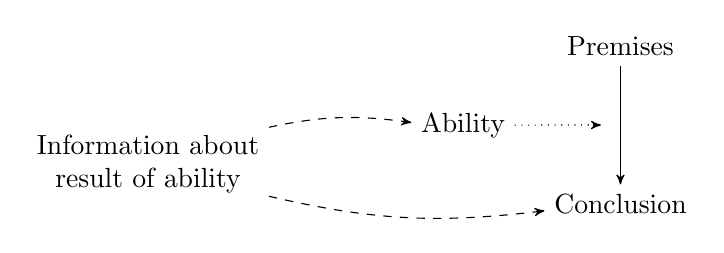
\begin{tikzpicture}[->,>=stealth',node distance=0cm, every text node part/.style={align=center}]

  \node (1) [] {Information about \\ result of ability};
  \node (2) [right of=1, xshift=4cm, yshift=.5cm] {Ability};
  \node (3) [above of=2, yshift=1cm, xshift=2cm] {Premises};
  \node (4) [below of=2, yshift=-1cm, xshift=2cm] {Conclusion};

  \draw [dashed, ->] (1) to [bend right=10] (4);
  \draw [dashed, ->] (1) to [bend left=10] (2);
  \draw [->] (3) to node[left] (mid) {} (4);
  \draw [dotted, ->] (2) to (mid);
\end{tikzpicture}
\caption{Sketch of support.
  Continuous arrow is direct.
  Dashed is indirect from information.
  Dotted is indirect from agent.}
\label{fig:dynamics}
\end{figure}


\begin{note}[Variation on a familiar problem]
  This is a twist on a familiar problem.
  Lots of ways to explain why an agent performed an action.
  Here, the agent is picking one of those ways.

  Problem is to identify the actual from the potential reasons.
  Here, our agent has a guarantee of potential reasons, and acts on the basis of those.
  If the agent could, then the agent is.

  With sufficient information about potential reasons, may an agent from appealing to those reasons when performing an action?

  justification footnote\nolinebreak
  \footnote{
    A different way to motivate the idea is through propositional and doxastic justification.
    As, the agent has a guarantee both that they are propositionally justified, and that they have the ability to be doxastically justified.
  }
\end{note}

Still, even though you would be able to demonstrate claim~\ref{chess:claim:2} without my testimony, my claim remains important in order for you to be confident that you have the ability --- even if you are confident that you understand the rules of chess and the game board, you would not be able to establish that White cannot prevent Black from occupying c4 on their second move without demonstrating a strategy for Black.
Claim~\ref{chess:claim:1} \emph{licenses} you to hold that claim~\ref{chess:claim:2} is true on grounds that are independent of my testimony.

Colloquially, you may cite the reasoning that you are able to do (or the strategy that would result from the reasoning) as support for holding that claim~\ref{chess:claim:2} is true.
And my testimony that claim~\ref{chess:claim:1} is true is then cited in support of your ability to do the reasoning.\nolinebreak
\footnote{
  Similar phenomena with `do you also hold \(\phi\) to be true?'
  Well, you hold \(\phi\) to be true, etc.
  So on the basis of you asking this, I may hold \(\phi\) to be true.

  Or, may reason to \(\phi\).
  So, alternative paths is not unique to ability attributions, though this differs in an important way, as you do not gain from this confidence that you can demonstrate that \(\phi\) is the case independently of the interaction.
}

  {
    \color{red}
    facts we take into consideration in reasoning are reasons \\
    reasons as items in pieces of reasoning, where reasoning is thought (or possible thought) directed toward some conclusion (\citeyear[421]{Hieronymi:2011aa})
  }
  Reasons that reasoning took into account, then a distinction between the reasons which led to the conclusion and the reasons that the agent takes to support the conclusion.


  Re-express the problem, the reasons why the agent holds that the Black has a strategy are those reasons that I (the agent) have the ability to reason with.

  This cuts across both `normative' and `explanatory' uses of `reason'.
  Why did the agent, in fact, act?
  If the agent is appealing to those witnessing reasons, then they are part of the explanation.
  If the agent is appealing to those witnessing reasons, then these affect whether the outcome was appropriate.

\hozlinedash

\section{Counterpart argument}
\label{sec:counterpart-argument}

The argument above is narrow.
Focused on the issue of whether or not the agent has support for a particular proposition.

Constrained so that the agent needed to endorse ability.
Hence could not obtain support.
These are the considerations I am inclined towards.
Support is important, but it does not necessarily need to be realised.

However, defensive.
May be that any realised support would do better.
The counterpart to the defensive argument is assuming that licensing is okay and suggesting when it may be preferred to realised support.

Scenarios, and then a big picture argument, where the big picture is different kinds of support.

\subsection{Failure Scenarios}
\label{sec:failure-scenarios}

\begin{note}[Failure scenario]
  Return to the logic classroom.

  \begin{itemize}
  \item If you are able to show \(\phi\), then by similar reasoning you are able to show \(\psi\).
  \item \(\phi \coloneq \exists x(Px \land Qx) \vdash \exists x(Px \lor Qx)\).
  \item \(\psi \coloneq \exists x (Px \land \exists x Qx) \vdash \exists x(Px \lor Qx)\).
  \item Student has some support for this --- whether the conditional holds isn't so important, so long as the agent is confident it does.
  \item The problem for the student is how the rules for instantiation work.
  \item Student isn't able to explain why the same instantiation on the two separate existential statements in \(\psi\) is bad.
  \item Tricky issue of whether the student really gets the antecedent of the conditional.
  \item Problem is that the result of luck doesn't seem to result in an ability.
  \item Still, sufficient grasp of working with single existential statements where no constants are involved.
  \item So I think it is fair to assume this --- if not, then things get difficult for most proofs --- not looking for mastery.
  \end{itemize}

  Student shows \(\phi\).
  Confident that the consequent holds.
  Hence, writes down \dots

  The student is correct, but the reasoning is not \emph{identical} --- different values for the distinct quantifiers.
  Instantiate, take the antecedent conjunction, and then introduce latter disjunct.
  Slight variation, and the student doesn't have the ability to show.

  This is suggested in a later proof, where the agent fails to appropriately use the rule.\nolinebreak
  \footnote{
    \begin{itemize}
    \item For example, \(Qa \rightarrow Ra, Pa, \exists x Qx, \forall x \lnot \exists y (x \ne y)\).
    \item Straight \(Qa\) for existential, with assumption of redundant premises.
    \end{itemize}
  }
  Let us stipulate that the student would obtain \(Pa \land \exists x Qa\).
  Rules governing quantifiers --- and quantifier scope --- are nuanced.

  Conditional doesn't hold because abilities are sufficiently distinct.
  Or, antecedent doesn't hold because success doesn't entail ability --- in contrast to exercising an ability, the student lucked the proof.

  Still, what the agent claimed is true, at least on a passable reading of `similar reasoning'.
  Instantiate the first existential, conjunction elimination, disjunction introduction, and existential generalisation.

  Student was unlucky, misled.
  Still, conditional/antecedent does not yield the conclusion without a factive inference from the agent's ability to show \(\psi\) by similar reasoning to the claim that \(\phi\) follows by similar reasoning.
  Misguiding confidence, but misguided confidence doesn't provide a complete picture.
  For example, thought it was going to be sunny today, but need to add that I left my umbrella behind to see how I was misguided.
  With the student, I claim, led the student to license reasons that they were not able to witness.\nolinebreak
  \footnote{
    May argue that the agent ought to have made the proof.
    Some fault for allowing student to make claims.
    Well, maybe.
    However, it seems as though ability statements can be used, and still have the problem of why the agent answered the problem in the way they did.
    And, agent was fine to be confident, hard to argue with this.
    If stakes are important, lower these as satisfactory.
    E.g.\ bonus problem, good grades, unneeded class, other things are more important, etc.
  }
  \hozlinedash

  The agent doesn't have the ability.
  The agent took the risk, and it didn't work out for them.
  The agent is not able to provide an explanation for the claim made.
\end{note}

\begin{note}[Factive reasons]
  This is somewhat similar to cases which suggest that reasons cannot be facts.
  Parallel in the sense that the agent needs to have the ability.
  Difference is the appearance/non-appearance of a reason.
  Similarity in the failure of an ability.
  However, if the similarity is pursued then difference is whether the agent possesses some input.
  Still, for now focusing on reasoning which involves explicit mention of ability.
\end{note}


\subsection{Three Positive Cases}
\label{sec:positive-cases}

\begin{note}[Cases]
  Here, deal with a number of cases.
  \begin{enumerate}
  \item Shopping \(\leadsto\) positing a simple relation between agents desire and action, tighten account of supporting reasoning.
  \item Detective \(\leadsto\) option of providing the support asynchronously.
  \item Temptation \(\leadsto\) agent's ranking of reasoning.
  \end{enumerate}
\end{note}


\subsubsection{Detective}
\label{sec:detective}

\begin{note}[Practical matters]
  I should include a note that the factive inference goes through, but it's up to the agent to figure out how to make use of this.
  Here, the potential may be insufficient.

  Similar, in some ways, to have evidence that would not be recognised by the court do to some administrative error (though this is not to say that not reasoning is the same as an administrative error).
\end{note}

\begin{note}[Async]
  Somewhere in here mention the idea of asynchronous reasoning.
  The reasoning doesn't (or reasons don't) necessarily stay potential.

  This ties to bounded agency, and part of the `why' question.
\end{note}

\begin{scenario}

  Case file contains evidence, but also notes made by Lewis.
  It is a mix, then, of the evidence that Lewis has gathered and inferences that Lewis has drawn.

  Morse looks through the case file.
  Does some reasoning.
  Makes use of the notes made by Lewis, so forms a conditional:

  \begin{itemize}
  \item If the case file is sound, then you are able to establish cause for bringing Woodthrope in for questioning.
  \end{itemize}

\end{scenario}

Morse provides information about an ability that Lewis has.


Note, this is not the same kind of conditional as in path 1.
For, the consequent of the conditional does not draw directly from an ability mentioned in the antecedent of the conditional.

Some remark on Lewis' ability is implicit, as notes are contained.
However, it does not follow that the reasoning demonstrated in these notes in the basis of Morse's claim.

The conditional could be false due to the ability claim.
The case file is sound, it does establish cause for bringing Woodthrope in for questioning, but Lewis does not have the ability to establish cause for bringing Woodthrope in for questioning.

Interest is in after the consequent is detached.
Lewis is confident that the are able to establish cause for bringing Woodthrope in for questioning.
Path 2, but the scope is a little different.
The reasoning made by Lewis is analogous.

The structure of the conditional is difficult for the two alternatives.
Morse has the ability, but Morse has not reasoned to the fact.
Similar considerations suggest that transforming Morse's claim into an assertion 

Lewis endorses Morse's evaluation of Lewis' ability.
Additional practical consideration --- Lewis needs to be confident that they are able to establish cause.



Reasoning is a little more complex.
Morse has provided a conditional --- Morse has not checked the inferences made by Lewis.
Lewis is in a position to endorse the case file --- evidence and inference alike, and then perform the factive inference.







Morse has done more reasoning, Lewis has done less.
More could be more helpful, and Lewis could be less reliant.



\subsubsection{Shopping}
\label{sec:shopping}

\begin{note}[Also include\dots]
  A note on having a stack of papers that one starts reading through.
\end{note}

\begin{note}[Difference between chess and shopping]
   The issue is that the agent hasn't worked through the reasoning --- \emph{not} that the agent is unaware of the reasoning required.
  This is an important distinction between the chess scenario and the shopping scenario.
\end{note}

\begin{note}[Main point]
  The key with this scenario is the simplicity of the explanation.
  If agent is in the clear, then this is because they have the supporting desire.
  If the agent is in a bind, then this is because they do not have the supporting desire.
  So, we don't need to fluctuate desires.

  Also something to the idea of an explanation.
\end{note}

The existence of chess strategies is, at least for most, uncommon and with little practical consequence.
Confidence of the ability, so can go to sleep, or as a way to provide assistance without providing novel information.
Also, two agents involved.

First scenario is common, practical consequence, and single agent.


\begin{scenario}[Shopping]

  Background:

  Friend recommends trying carambola.
  Agent forms a desire.
  Does some research.
  Carambola and star fruit are the same thing.
  Hence, desire for star fruit.
  Purchasing as a means to this end.
  Writes a note on the shopping list.

  Out shopping.
  Sees star fruit.
  Does recall carambola.
  Does not recall that carambola and star fruit are the same thing.
  Confident that they are able to reason from a desire that they have to purchasing star fruit.
\end{scenario}

\begin{note}[Required conditions]
  Here, the shopping list provides the first required condition, and some nebulous considerations support confidence that the agent has the ability to do the reasoning again.
\end{note}




\subsubsection{Weakness of will}
\label{sec:weakness-will}

\begin{note}[Idea]
  This combines idea from the previous two.
  From shopping, the idea of preferable explanations, but now from the viewpoint of the agent.
  From detective, the idea of providing the appropriate reasoning at an other point of time, here from the past --- or potentially the future/counterfactual perhaps.
\end{note}

\begin{note}[Counterfactual]
Also could be framed as counterfactual ability.
Cases of rational impairment and so on.

In a sense, the issue here is the strength of the conclusion.
It seems the conclusions obtained while sober often extend and hold when intoxicated.

However, by contrast, conclusions obtained with full information may not.
E.g.\ \cite{Smith:2004aa} or the miners paradox.
\end{note}


\begin{note}[Different types of reasoning]

  The reasoning performed by the agent may be characterised as the \emph{preservation of a designated value}, where the designated value is \emph{truth}.
  For, if certain premises are true, then the conclusion is also true.

  This is distinct from the reasoning that the agent is able to perform, which may be characterised as the \emph{construction of a witness}.\nolinebreak
  \footnote{
    The relation here is similar to a position advocated by \citeauthor{Prawitz:2005aa}:
    \begin{quote}
      In the same vein, the assertion of a sentence is understood constructively as the claim that there is direct evidence for it, and is to be taken as true if such evidence exists.
      In mathematics the truth of a sentence thus becomes equated with the existence of a canonical proof or argument for it.\nolinebreak
      \mbox{}\hfill\mbox{(\citeauthor[692]{Prawitz:2005aa})}
    \end{quote}

    A nice quote from \textcite{Broome:2013aa}:
    \begin{quote}
      Facts that merely entail that an agent ought to perform the action are not necessarily reasons for her to perform it; to be reasons they must explain why she ought to perform it.\nolinebreak
      \mbox{}\hfill\mbox{(\citeyear[51]{Broome:2013aa})}
    \end{quote}
  }\(^{,}\)
  \footnote{
  To help illustrate the difference between the preservation of a designated value and the construction of witnessing reasoning, consider what Achilles said to the Tortoise:
  \begin{enumerate}[label=(\emph{\Alph*}), ref=\emph{\Alph*}]
     \setcounter{enumi}{2}
    \item\label{achilles:C} If~\ref{achilles:A} and~\ref{achilles:B} and true,~\ref{achilles:C} \emph{must} be true.
  \end{enumerate}
  Where A, B, and Z are:
  \begin{enumerate}[label=(\emph{\Alph*}), ref=\emph{\Alph*}]
  \item\label{achilles:A} Things that are equal to the same are equal to each other.
  \item\label{achilles:B} The two sides of this Triangle are things that are equal to the same.
    \setcounter{enumi}{25}
  \item\label{achilles:Z} The two sides of this Triangle are equal to each other.
  \end{enumerate}
  The Tortoise does not accept~\ref{achilles:C}, though the Tortoise does accept that~\ref{achilles:A} and~\ref{achilles:B} are true.
  The response of Achilles, \ref{achilles:C}, asserts that truth is preserved when moving from~\ref{achilles:A} and~\ref{achilles:B} to~\ref{achilles:Z}.
  Still, even if truth is preserved from~\ref{achilles:A} and~\ref{achilles:B} to~\ref{achilles:Z}, the Tortoise has a point --- preservation of truth is only useful is there is a guarantee that truth is in fact being preserved, and \emph{If you accept~\ref{achilles:A} and~\ref{achilles:B} and~\ref{achilles:C}, you must accept~\ref{achilles:Z}} is no more of a guarantee that~\ref{achilles:Z}.
  Carrol doesn't say --- or Achilles does not attempt to see -- what the Tortoise would have made of the following (sketched) reasoning.
  \begin{itemize}
  \item Let two sides of this triangle be labelled \(s_{1}\) and \(s_{2}\).
  \item As~\ref{achilles:B} is true, we know that there is some thing, say \(s_{e}\) equal to both \(s_{1}\) and \(s_{2}\).
  \item As both \(s_{1}\) and \(s_{2}\) are equal to \(s_{3}\), we see by~\ref{achilles:A} that \(s_{1}\) and \(s_{2}\) must be equal to each other.
  \item Therefore~\ref{achilles:Z} is the case.
  \end{itemize}
  The Tortoise may object to a step in this reasoning, though it is unclear whether they would as Achilles insists on convincing the Tortoise that~\ref{achilles:Z} must be true when~\ref{achilles:A} and~\ref{achilles:B} are true without working through the relation between the contents of~\ref{achilles:A} and~\ref{achilles:B} and the contents of~\ref{achilles:Z}.
  Perhaps the Tortoise does not accept that the two sides of the Triangle are equal to each other, or perhaps the Tortoise is seeking a demonstration of why the two sides of the Triangle are equal to each other that follows from the contents of~\ref{achilles:A} and~\ref{achilles:B}.

  So, one may hold that~\ref{achilles:C} is of interest only to the extent that certain things about equality and this Triangle conspire to make it so that the two sides of this Triangle are equal to each other.
  These things can be ignored if one grants that there is preservation of truth from~\ref{achilles:A} and~\ref{achilles:B} to~\ref{achilles:Z}, but the preservation of truth follows from those things, and can not be substituted for them.

  Hence, the Tortoise may refuse to accept~\ref{achilles:C} so long as the Tortoise is unclear on how equality and this Triangle are related, as the preservation of truth is merely a byproduct of whatever that relation is.
  The (sketched) reasoning, in turn, provides the Tortoise with an account of what truth is, at least with respect to these premises

  (Note that this is analogous to the rules of chess, game state, and possibility in the opening scenario.)
    {
    \color{red}
    \begin{enumerate}[label=(\emph{\Alph*\('\)}), ref=\emph{\Alph*\('\)}]
    \item\label{Achilles:Chess:A} Starting with game state and following the rules of chess.
    \item\label{Achilles:Chess:B} Black moves from d7 to e5 and then from d7 to c4.
      \setcounter{enumi}{25}
    \item\label{Achilles:Chess:Z} Black has occupied c4 without an opportunity for White to prevent Black from occupying c4.
    \end{enumerate}
    Hence:
    \begin{enumerate}[label=(\emph{\Alph*\('\)}), ref=\emph{\Alph*\('\)}]
      \setcounter{enumi}{2}
      \item\label{Achilles:Chess:C} If~\ref{Achilles:Chess:A} and~\ref{Achilles:Chess:B} are true, then~\ref{Achilles:Chess:Z} must be true.
    \end{enumerate}
    And so on\dots
  }
}

  Simply put, the reasoning that the agent performed guarantees that a strategy for Black exists as it must be true that a strategy for Black exists (if certain premises are true).
  The reasoning that the agent is able to perform, by contrast, would provide a particular strategy for Black, a witness for the existential statement that a strategy for Black exists.

  So, if the agent holds their ability as support, then this is a different kind of reasoning from the reasoning they performed.

  I am inclined to treat the construction of a witness as something more important, but for present purposes it is a contingent feature made to illustrate.
  Here, simple observation that the support is different.
  If the agent appeals to the reasoning that they are able to do in support, then the agent is appealing to support that differs from the reasoning they have performed.

  If so, then from the agent's point of view there is a divergence between the reasoning that led to the conclusion and the reasoning which supports the conclusion.

  {
    \color{red}
    It is important that these types of reasoning differ.
    However, it is only important in so far as the provides a way to distinguish and motivate interest in the reasoning that the agent is able to do.
    Motivate as intuitively there is something else, and distinguish as a clean line helps (in what way?)
    There may be cases in which the agent's ability to preserve a designated value is of interest.
  }
\end{note}

\section{Resistance}
\label{sec:resistance}


\subsection{Voluntarism and Hobson's Choice}
\label{sec:non-voluntarism}

\begin{note}[Grr]
  I think this belongs in the objection section, which might also help with structure.
  For, the worry here is that licensing reasoning is a form of voluntarism.
  One the one hand, I do not claim that the result of licensing is belief.
  Still, it seems to me this is relatively open --- functionally similar.

  Idea would be that reconstruct \citeauthor{Weatherson:2008uq}, hence obtain that licensing is voluntary, and therefore there is a problem with applying the factive inference?
  For, this involves a choice made by the agent, and that goes on to block any factive inference where the proposition is suitably independent.

  This is also somewhat suggested by the \citeauthor{Davidson:2001aa} motivation, where in a way there's a suggestion of the agent picking the reasons to believe something ---- however this in part focuses on the why and not the which.

  This is not to say that it is not possible for the agent to make the factive inference, but that it is not sound to do so.
  Right, kind of get the intuition that the agent would withdraw the factive inference if they were to reconsider the possibility that the carton in the fridge is empty.

  Then, the response is that it is a mistake to think that exercising the capacity is important in these cases.
  For, to the agent there is no issue of self control.
  For, in these cases the agent is confident that things would not go otherwise.
\end{note}

\begin{note}[Broad outline]
  The debate around voluntarism is difficult.
  What belief is, what voluntarism requires, whether cases can be excluded, etc.\
  Hence, unclear on what one obtains by voluntarism.
  Whether one has control over doxastic states.
  Whether there are deontic parallels between beliefs and actions.
  Understanding of justification.

  I am not inclined to take an absolute position, but I think that ability limits any voluntarist position in which failure to exercise a capacity to reason amounts to a voluntary act.

  Here, \citeauthor{Weatherson:2008uq}.

  \begin{quote}
    These conclusions that we leap to are voluntary beliefs; we could have avoided forming them.
    And not only could we have avoided these formations, but we would have if we had followed the methods for belief formation that we approve of.
    That seems enough, to me, to say the formation is voluntary.\nolinebreak
    \mbox{}\hfill\mbox{(\citeyear[10]{Weatherson:2008uq})}
  \end{quote}

  Checking the fridge, keeping counterexamples in mind, and so on.
  \citeauthor{Weatherson:2008uq}'s argument, roughly, is that these cases involve failure to exercise a capacity, and whether to exercise the capacity to reason is up to us.

  Argument, roughly, is that if an agent is confident in their ability to reason, then the agent is confident that they could not have avoided forming them.

  Obtaining a conclusion by licensing reasoning is not the same as failure of self-control.


  Extreme cases, like \citeauthor{Ginet:2001aa} I have nothing to say about.
  However, cases such as those suggested by \citeauthor{Weatherson:2008uq}.
  Here, following approved methods is not so clear.
\end{note}

\begin{note}[The factive inference]
  I do not assume that the factive inference results in belief.
  \url{https://iep.utm.edu/doxa-vol/} has relies on Ginet, where acceptance or acting as if true seems appropriate.
  And, I think so parallels could be drawn between my cases and those Ginet discusses.

  So, this provides a kind of voluntarism, but suggests a finer issue than Ginet notes.
\end{note}

Interested in inferential \(\phi\) for which the factive inference can be made.

Plausible link:
\begin{enumerate}
\item Agent may believe \(\phi\) only if agent is able to reason to \(\phi\).
\end{enumerate}

Stronger:
\begin{enumerate}
\item Agent may believe \(\phi\) only if agent is confident that they are able to reason to \(\phi\).
\end{enumerate}

The `may' of the antecedent can be read as rational permissibility, etc.

Indirect argument is that an agent is able to believe \(\phi\) only if the agent has reasoned to \(\phi\).
Therefore, it seems the agent must be confident that they are able to reason to \(\phi\), as if the agent is not confident that they have witnessed their ability, then the agent would doubt that \(\phi\) is the case.
So, this isn't interesting if an agent believes that \(\phi\).

However, this won't do for investigating voluntarism.
First issue is that choice may be part of the reasoning the agent is confident that they are able to do.

So, the appropriate reading of reasoning here needs to exclude choice.
Yet, in doing so this assumes that voluntarism is false.


\begin{enumerate}
\item If it is not the case that an agent is confident that they are able to reason to \(\phi\), then it is not the case that the agent may believe \(\phi\).
\end{enumerate}

\begin{note}[Justification]
  The key idea with \citeauthor{Ginet:2001aa} is that sometimes a person was not justified in holding a belief.
  And, this seems to entail that the person had the choice to make the belief.

  This, then, is similar with \citeauthor{Weatherson:2008uq}, where justification is optional.

  So, justification, therefore voluntarism.

  Quick argument is:

  \begin{enumerate}
  \item (Agent was not justified.)
  \item Agent ought not have.
  \item Agent could not have.
  \item Agent had a choice.
  \end{enumerate}
  Therefore, voluntarism, at least in some cases.
  \citeauthor{Ginet:2001aa} is somewhat explicit about this.
  \citeauthor{Weatherson:2008uq} is similar, something the agent ought to have done, and therefore the agent had a choice.

  With \citeauthor{Ginet:2001aa} we have lack of justification.
  So, if a requirement of justification is placed for rational belief, then these cases are going to fail.
  With \citeauthor{Weatherson:2008uq} we have partial justification.
  And, as this is non-monotonic, same idea.

  Inclined to agree that the agent had a choice.
  However, it does not follow from this that it appeared to the agent that they had a choice.
\end{note}

\begin{note}[Weatherson]
  It seems that \textcite[10]{Weatherson:2008uq} suggests that we leap to these conclusions, and that if we follow reasoning patterns that we approve of, then we would not perform these leaps.
  Hence, a key part of the argument for these being voluntary (though not volitional) is that these inferences are akin to losing one's temper.

  However, if ability is added, then these are not cases similar to losing temper.
  For, one is not failing to perform some reasoning that would otherwise be done, but taking a license for the reasoning.
  The agent makes a mistake in licensing these reasons, but this, I think, blocks some of the appeal of the argument.
\end{note}

\begin{note}[Link to belief]
  Hence, \citeauthor{Ginet:2001aa} isn't quite correct.
  The agent is able to reason to at most one, and it is a mistake to think otherwise.
  Still, \citeauthor{Ginet:2001aa}'s diagnosis is on point --- the agent does \emph{stake} something.

  \begin{quote}
    There are all sorts of beliefs that we form in haste, where we could have stopped to consider the various realistic hypotheses consistent with the evidence, and doing so would have stopped us forming the belief.\nolinebreak
    \mbox{}\hfill\mbox{(\citeyear[10]{Weatherson:2008uq})}
  \end{quote}
  Here, and in the following, \citeauthor{Weatherson:2008uq} focuses on exercising a capacity.

  However, there is a contrast with \citeauthor{Weatherson:2008uq}, who assumes, it seems, that the agent has performed sufficient reasoning, and questions whether the agent `should have' performed more reasoning.
  This then really does seem to be a case of voluntarism, as the agent decides where to stop, but going further may reverse the evidence --- but then unclear why this doesn't also apply to perceptual experience, as this may also be cut short.

  Also issue of how things appear to the agent.
  Noting that things could have gone otherwise doesn't seem compelling.
  Argue that here the agent was either irrational or did not observe a choice.
  So, \citeauthor{Weatherson:2008uq} may be right, in that things could have gone otherwise, but it's hard to square this with \emph{choice}.
  In a sense, the agent made a choice, but it seems something of a Hobson's choice.

  The point about perceptual beliefs is somewhat interesting.
  Need a case in which one could have avoided seeing something.
  So, think of an optical illusion, two lines appear to be the same length.
  Option of not seeing this.
  It is not clear to me where the difference is.

  However, this is achieved is by way of uniqueness.
  When there are multiple options, the same principle applies, but without much consequence.
  E.g.\ choosing cereal.
\end{note}

\begin{note}[Main idea]
  The point about non-voluntarism can be held independently from the broader point that I want to make.
  For, this is about restricting the choices of an agent, rather than providing the agent with choices, roughly stated.
  Hence, lack of ability make block, but it does not follow from this that instance of abilities opens.

  \begin{itemize}
  \item \emph{Therefore} I don't have anything robust to say about \emph{doxastic} voluntarism.
  \item Still, in these cases it's not clear that there is really voluntarism.
  \end{itemize}

  However, similarity in the sense of potential reasoning.
\end{note}

\begin{note}[What voluntarism is]
  The basic idea with non-voluntarism is that the agent does not have the option to form certain propositional attitudes.
  Primary case is belief --- \emph{doxastic} voluntarism (though the general idea extends to any attitude which may be the conclusion of reasoning).
  Motivating example: ???
\end{note}

\begin{note}[Something odd]
  Here, there's some odd.
  For, if focus is on cases where the agent does not have the ability, then this doesn't provide support for holding the opposing attitude.
  Unless, one has an exclusive disjunction.

  So the core idea here is that because the agent doesn't have the ability for, say, the negation, the agent does not obtain the particular attitude by volition.
  So, the key here is thinking in terms of conclusions of reasoning.
  Non-voluntary because exclusive conclusion, and the agent does not have the ability to reason to one of these.
  Doxastic stuff is interesting then, because it seems there is a unique attitude determined by the agent's evidence, whether belief, suspension, or disbelief.
\end{note}

\begin{note}[Hum]
  So the idea behind this kind of non-voluntarism is that the agent doesn't have the ability to reason to a particular conclusion.
  However, this isn't a good account of non-voluntarism and it doesn't say anything about what the agent does reason to.
  So, choosing breakfast cereals at the supermarket.
  Don't have the ability to reason to the conclusion that some particular cereal is any good.
  However, whatever cereal I do choose, it seems I do so voluntarily.
\end{note}

The main focus of the paper has been indirect access to reasons.

With non-voluntarism, the same ideas apply, but rule out certain conclusions.

It's the denial of an existential.

If the existential provides access and allows a conclusion to be adopted, and this holds in converse, then we've got a clear account of when an agent does not have the option of adopting a conclusion.

Hmm, there are two instances of this claim:
\begin{enumerate}
\item Adoption requires ability, hence if no ability then no option to adopt.
\item Ability along with exclusivity rules out certain options.
\end{enumerate}


\subsection{Different types of reasoning}
\label{sec:diff-types-reas}

\begin{note}[Idea]
  The goal here is to broaden the basic idea that there are preferable explanations in many cases.
\end{note}

\begin{itemize}
\item \emph{Reasoning just is the preservation of a designated value}.
\item The designated value is true, utility, etc.
\item If this is so, then there's nothing more.
\item This is a strong argument, as nothing (of interest) can be gained by generating the additional reasoning.
\end{itemize}

\begin{itemize}
\item \emph{This is may be quite standard.}
\item Think about practical reasoning.
\item Means-end, in particular, and how necessity is invoked.
\item The supermarket is useful here, as on one reading, I have shown that I must buy the star fruit, but on another reading I have demonstrated why buying the starfruit would do something for me.
\end{itemize}

\subsection{Full explanations, so to speak}
\label{sec:full-explanations-so}

\begin{note}[Idea]
  Observe the general kind of problem with extant accounts of reasoning and show that these can be seen as true when certain restrictive conditions are in place.
\end{note}


\begin{note}[Generator]
  Now, the existence of the license does some work in the causal explanation, so to speak.
  It is part of the reasoning that the agent does.
  The issue is about how it fits, with the idea being that one needs to turn it on (figuratively) to get the support that the agent cites, or the justification for the agent's action.
\end{note}

\subsection{Internalism and externalism}
\label{sec:intern-extern}

\begin{note}[License]
  Need assurance that license is good.
  Hence, the role of the agent's ability.
  I assume that the agent's ability is involved.
  This may be redundant.
  Difficult.
  Distinction between internal and external reasons.
  Ability makes this a little fuzzy, and this is why there is appeal.
  Supports the idea that these would function as internal reasons.
  If the agent does not have the ability, then the same may still hold.
  For example, passing reasons between agents.
  Agent A grants agent B license to appeal to the reasons that agent A has in order to agent B to obtain a result.
  Etc.
\end{note}

\begin{note}[Maybe?]
  Can I make use of a distinction between \emph{potential} reasoning and \emph{external} reasons?
\end{note}

\begin{note}[Supervenience]
  Perhaps restructure some of the supervenience observations here.
  I.e.\ because we're interested in reasoning ability, it seems this may be compatible with supervenience.
  For sure, the claim is restricted in this way.
  If agent appeals to explanations \emph{other} than their ability to reason, then it seems plausible that supervenience may fail.
  However, this is independent of the focus point, and may be taken up elsewhere.

  I mean, in short, if the intuition goes via twin duplicates, then it seems as though these should have the same reasoning ability.
\end{note}

\section{License}
\label{sec:license}


\begin{note}[Constructive]
  An important point here is that the agent's reasoning is non-constructive, in a sense.
  For, the agent has a guarantee that the conclusion is true, but the agent does not establish \emph{why} the conclusion is true.
  Hence, there are (at least) two `why' questions.
  \begin{itemize}
  \item Why the conclusion follows from the premises (and the agent's ability), and
  \item Why the agent holds the conclusion to be true.
  \end{itemize}
  If the agent were to do the reasoning, then these would both be answered.
  The explanation of why the agent holds the conclusion to be true (from the agent's point of view) is the same explanation as to why the conclusion follows from the premises.

  Something like, knights can move \dots, the knight can be captured only if \dots, the knight cannot be captured.
  White can only move to \dots, etc.\

  So, we can see that the agent has the ability to answer the first question --- why the conclusion follows from the premises.
  However, because the agent has not done the reasoning, this does not answer the second question.

  Still, the agent's ability guarantees that an answer to the first question may be generated by the agent.
  This is reminiscent of \citeauthor{Davidson:2001aa} \dots
\end{note}


\begin{note}[Davidson]
  \begin{quote}
    Because justifying and explaining an action so often go hand in hand, we frequently indicate the primary reason for an action by making a claim which, if true, would also verify, vindicate, or support the relevant belief or attitude of the agent.

    \vdots

    The justifying role of a reason, given this interpretation, depends upon the explanatory role\dots
    \nolinebreak
    \mbox{}\hfill(\cite[8]{Davidson:2001aa})
  \end{quote}

  If \citeauthor{Davidson:2001aa} is followed, then justification only if explanation, and explanation only if causation.
  So, justification only if causation.
  But this presents a problem.
  For, the agent's ability has not been witnessed, and therefore the justification that would be constructed cannot stand in any causal relation to the agent adopting an attitude toward the conclusion.

  The idea expressed above mirrors the interaction \citeauthor{Davidson:2001aa} points to.
  For \citeauthor{Davidson:2001aa}, justification indicates how to construct a primary reason which explains.
  In our case, primary reason indicates how to construct justification.

  So, this is a problem.
  {
    \color{red}
    Either the agent's ability does not do any justificatory work, or there is justification without causation.
    \emph{However}, this misses an alternative.
    The justification isn't the focus.
    It's the guarantee of justification.
  }
  The first option may be preferred.

  Have some reasoning, seems okay.
  Therefore, this provides justification.
  I struggle with this.
  The agent's reasoning obtains a guarantee of truth.
  However, this is `simply' \(\phi \rightarrow \psi\), without understanding why \(\phi \rightarrow \psi\).

  Contrast to a simple model of testimony.
  You have justification.
  Hence, the hearers justification goes by way of the speakers justification.

  The details of causation matter.
  However, abilities (or what would result from abilities) avoid some of the issues here.
  For, nothing is witnessed.

  It is somewhat interesting that \citeauthor{Davidson:2001aa} emphasises that one often doesn't have the primary reason, and instead provides information that is sufficient to generate the primary reason.

  So, the idea that an explanation can be generated is stressed by \citeauthor{Davidson:2001aa}.
  Difference is that \citeauthor{Davidson:2001aa} makes use of this idea when providing information about explanations.



  \begin{quote}
    Central to the relation between a reason and an action it explains is the idea that the agent performed the action \emph{because} he had the reason.
    Of course, we can include this idea too in justification; but then the notion of justification becomes as dark as the notion of reason until we can account for the force of that ‘because’\nolinebreak
    \mbox{}\hfill(\citeyear[9]{Davidson:2001aa})
  \end{quote}
\end{note}



\subsection{Ability}
\label{sec:ability}

\begin{note}[Issues with simply talking about ability --- verifying vs.\ solving]
  Similar to calculators.
  \(7^{3} = 343\), but I do not consider the result of computer program a reason to hold that \(7^{3} = 343\).
  The program informed me that, given my understanding of arithmetic, I may hold that \(7^{3} = 343\).

  Compare to:
  \(\lim_{n \to \infty}\left(1 + \frac{1}{n} \right)^{n} = e\)
  This goes beyond my ability.
  If the computer program provides an explanation of how the result was derived, I may study the steps and identify ways to develop the ability, e.g.\ by developing an understanding of l'H\^{o}pital's rule.

  While there is an intuitive distinction between the ability to show that \(7^{3} = 343\) and the ability to show that \(\lim_{n \to \infty}\left(1 + \frac{1}{n} \right)^{n} = e\), there are intermediate cases which put pressure on what is meant by the ability to reason from \(\Sigma\) to \(\phi\).
  For example, I doubt I have the ability to solve \(\sqrt[5]{59049}\) without some assistance, but I do have the ability to show that \(9^{5} = 59049\), and hence the ability to verify that \(\sqrt[5]{59049} = 9\).

  I consider both the ability to solve and the ability as instances of ability to reason, but keeping track of the differences is not too important.
  Therefore, to keep things simple I take talk of the ability to reason to align with the ability to solve.
\end{note}



\subsection{Mental state}
\label{sec:mental-state}

{
  \color{red}
  The main idea, really, is that I end up `wrapping' many principles in a conditional of the form:
  \begin{quote}
    If full explanation then (\emph{Principle})
  \end{quote}
  So, if you're into a particular principle, you get to keep this principle, so long as you don't also hold that the principle is sufficient for a full explanation.

  It seems, perhaps, the most will not hold the converse.
  For, cases of deviance.
  Deviance also helps to demonstrate the general use of a wrapper --- restrict to particular cases.
  However, one may wish to drop the `full' from the wrapper, and claim the principle holds whether an explanation is available.
}

I think, potentially, that a number of these objections can be grouped under the idea of a reason or reasoning being a mental state.

\subsection{Actual reasoning}
\label{sec:actual-reasoning}

\begin{note}[Ability]
  Distinction between:
  \begin{itemize}
  \item The agent's ability.
  \item The property of the agent that they have the ability.
  \end{itemize}
  This is an important distinction.
  The agent's ability is not, in general, a property of the agent.
  Ability involves actions/events.
  But these can be referenced by a predicate.

  So, the structure between the premises and conclusion is done by the ability, not the property.

  This is `the factive inference'.

  Still, one may distinguish between the fact and the considerations which result from a factive inference.
  This is fair.
  And, this allows us to some flexibility.
  However, there is a difference between the fact and the considerations.
  For, the considerations have partial information, while the fact \emph{is} the information (speaking loosely).
  So, it does not seem possible to completely move away from the agent's ability.
\end{note}

\begin{itemize}
\item Objection is that the agent's confidence in their ability is `enough' of an explanation.
\item Reminiscent of an idea from Williamson, and recently put to use by \citeauthor{Lord:2018aa} (and maybe \citeauthor{Kiesewetter:2017aa}).
\item Here, the factive entailment is enough for an explanation, very roughly.
\item In this way, one can explain by appearances, and this does enough.
\item However, the issue is with the \emph{kind} of explanation that is obtained.
\item The factive inference gets a truth-truth/non-constructive explanation.
\item The conclusion must be true, but this does not constructively explain why the conclusion is true.
\item So, this doesn't really do anything, and the same issue arises for this kind of explanation.
\item The inference is truth-truth, with the assumption of something else doing the work.
\end{itemize}

\begin{note}[The Williamson idea]
The Williamson idea is that it's reasonable to hold that appearance is factive.
Hence, \citeauthor[Ch.\ 7]{Lord:2018aa} and \citeauthor{Kiesewetter:2017aa} are able to argue that appearances provide reasons.
Not necessarily the same (kind of) reasons, but sufficient reasons.

(
As an aside, this is somewhat interesting because it provides an account of why appearances are reason-giving.
One could argue that this is independently true, but the interesting point is that objective reasons are non-redundant even if they are reason giving.
For, if there were no objective reasons then there would not be an entailment from appearance to reason.
)

The strategy doesn't apply to the cases that I am interested in.
For, this would require me that the agent's confidence in their ability provides a reason.
However, the natural understanding of the scenarios is that the agent relies on their ability to guarantee the existence of a reason, rather than the ability \emph{itself} being a reason.
\end{note}

\subsection{Causation}
\label{sec:causation}

The core idea here is that causation is only going to work if one thinks that the agent's reasoning provides a `complete' explanation.
I deny that the agent's reasoning provides a complete explanation --- the point of licensing is to secure a `complete' explanation without doing the reasoning.

Basically, the agent's reasoning needs to be part of the causal chain.

\subsection{Supervenience}
\label{sec:supervenience}

The idea is that supervenience is stronger than appealing to causation, because we have an argument for why the \emph{content} is not part of the explanation when appealing to supervenience (or the dependency strengthened version of supervenience).

I can't simply argue that there is more to the explanation, because if supervenience holds then there cannot be anything else.

\begin{note}[Structure]
  Overview of section:
  \begin{itemize}
  \item Supervene on internal mental states.
  \item This is a problem, as the agent's potential reasoning is not an internal mental state, seems one can vary ability without changing anything --- certainly true in general cases of ability.
  \item Whether this holds for reasoning in particular is unclear.
  \item Note, however, two kinds of supervenience.
    \begin{itemize}
    \item Reasons,
    \item Rationality
    \end{itemize}
  \item Interested in supervenience of reasons.
  \item The idea is that this rules out the agent's potential reasoning as being something that explains.
  \item It cannot stand in the role of a reason because the potential reasoning does not supervene.
  \item Plausible that ability supervenes, if supervenience is characterised broadly, which it may need to be.
  \item Arguably, this does not address the motivating intuition.
  \item As an aside --- in principle, supervenience is compatible with externalism about mental content, and one may argue that the licensing pulls in the reasoning in this way.
    \begin{itemize}
    \item Still, ability can vary without confidence in ability varying --- this subdivides the agent's mental states, but holds on to the same intuition.
      For, the agent's reasoning would go through without this --- the key is that supervenience establishes a kind of dependency relation, and the idea is that anything outside of this dependency relation is not required for an explanation.
    \item This entails supervenience, but is a little stronger.
    \item Supervenience is a particular kind of dependency relation, no?
    \item If one took up the aside, then we find that the external content would be redundant, only some of the state matters.
    \end{itemize}
  \item So, this provides an argument for the idea that the agent's potential reasoning being redundant.
  \item The argument isn't perfect.
    For, there are cases where it doesn't seem as though one can strip away redundancy --- e.g.\ \(p, p \rightarrow q, q \rightarrow r\) hence \(p \rightarrow r\) by conditional proof and hence \(r\) versus detaching the way through --- as one has already done this in the conditional proof so it seems redundant.
    Still, I take the broad strokes to be sufficiently clear.
  \item A consequence of this is that by using something in reasoning it becomes a reason.
  \item The agent is going to get to the conclusion whether or not they have the ability.
  \item Evil demon cases.
    \begin{itemize}
    \item We see that the agent only needs the relevant premises.
    \item But, may not need the demon.
    \item Example where premises of reasoning may no longer hold.
    \item May think that this is the same as, for example, memory, where the thing remember may no longer hold.
      However, here we often take memory itself to be the source, not the thing remembered.
      Licensing suggest this need not be the case, but the problem remains.
    \end{itemize}
  \item So, the agent's ability is not a premise, only the agent's confidence that they have the ability is a premise.
  \end{itemize}
\end{note}

\begin{note}[Main points]
  Supervenience is an interesting take.
  Need to show that the potential reasons do not supervene.
  This is not obvious.

  The simplest way to object to this is to note that what the agent has an ability to do varies given other things.
  Some easy examples of this, such as the arrangement of tennis players in a tournament.
  The order of play may determine whether or not the agent has the ability to reach the grand final.
  As, particular adversary, but they're weak to another player, that the agent is strong against.
  Hence, the draw may work out in the agent's favour.

  Does the same phenomena arise with reasoning?

  There's also the issue of factivity, which \citeauthor{Singh:2019aa} notes.

  The way I \emph{want} to object to this is to claim that the agent does not, in the appropriate sense, have a motivating reason.
  The agent \emph{needs} the factivity to get the motivation.
  Hence, without this there is no reason to speak of.
  There's nothing to `get' from the agent's motivating reason.
  This restricts the scope of supervenience, in a sense.
  Not all reasons that motivate explain, or not all reasoning explains.
  (Not: not all reasons are motivating reasons --- not all reasoning is motivates.)
  Some ideas of \citeauthor{Lord:2018aa} seem to apply here --- some of our judgements about rationality apply, but not all.

  The above restricts the application of supervenience.
  An alternative is to argue that ability to reason does supervene on the mental.
  Hence, superveniece does not fail.
\end{note}

\begin{note}[Two superveniece claims?]
  Is there a distinction between the claim that reasons supervene and the claim that rationality supervenes?
  Possible, if rationality is insensitive to whether or not something is genuinely a reason.

  \begin{itemize}
  \item Rationality involves responding to reasons, etc.\
  \item Rationality is about structure, and whether or not structure is supported depends on ability.
  \end{itemize}

  The difference really does seem important.
  For, there are factive inferences all over the place, but if we restrict attention to the reasoning involved, then nothing goes beyond this.
  By analogy, it's the difference between validity and soundness.
  This is kind of what \citeauthor{Lord:2018aa} gets at with the idea of comparative rationality.

  So, the issue here is whether the agent has the same reasons in both cases.
\end{note}


\textcite{Singh:2019aa} has an extended discussion of supervenience.

\begin{quote}
  \textbf{Supervenience Constraint (SC)}: an agent’s motivating reasons supervene on the internal facts about her mental states.

  \vdots

  The internal facts about agents’ mental states are the facts about their non-factive mental states and the relations between them\nolinebreak
  \mbox{}\hfill\mbox{(\citeyear[6]{Singh:2019aa})}
\end{quote}

\citeauthor{Singh:2019aa} notes that this does not entail that nothing about an agent's motivating reasons can change without a correspond change in the agent's mental states.
For, it may be the case that a motivating reason switches between \emph{also} being a normative reason, depending on what the facts of the situation are.

{
  \color{red}
  There's also \citeauthor{Broome:2013aa}'s claim that rationality supervenes on the mind (\citeyear[151, etc.]{Broome:2013aa}).
}

\begin{quote}
  One such starting point, which I hope is uncontroversial, is that an agent’s motivating reason must play a motivational role (broadly understood) in her psychology.
  If it did not play this role in her psychology (that of motivating her, in a broad sense) it would not be her motivating reason.
  Thus, whatever a motivating reason is, it must be something that can play this psychological role.\nolinebreak
  \mbox{}\hfill\mbox{(\citeyear[4]{Singh:2019aa})}
\end{quote}

\begin{note}[Compatibility]
  First point is compatibility.
  Agent's ability to reason, perhaps this supervenes.
  Plausible, but this doesn't get to the real objection here.
  Ability may supervene, but agent's confidence may not.
  And this is where the problem starts.
  For, even if the ability supervenes, it's the confidence that the agent has the ability that does the work.
  And \emph{this confidence} does not supervene on the ability.
  The reasoning that the agent does is the same in both cases, even as we move around whether or not the agent has the ability.
\end{note}

\begin{note}[Motviation for supervenience/evil demons]
  The standard motivation for supervenience seems to be evil demon type cases.
  Here, factivity fails, intuitions about reasons remains roughly the same.
  Hence, factivity is not a principal component of the analysis, at least.

  \citeauthor{Singh:2019aa} has a nice line which links up to reasoning:
  \begin{quote}
    \dots since you reason exactly the same way to the exact same beliefs and actions, it remains the case that your motivating reasons are the same in both worlds.\nolinebreak
    \mbox{}\hfill\mbox{(\citeyear[5]{Singh:2019aa})}
  \end{quote}
  The intuition is that the reasoning would be the same.
  But this is tricky, and exactly where the distinction comes into effect.
  Agent's reasoning supervenes, but we need to stipulate that the agent's reasoning would be different if their reasons were different.
  If the demon cases hold, then whether or not a given mental state is factive is independent of whether or not an agent applies a factive inference to that mental state.
  Separate whether or not something is a reason from the use it has in the agent's reasoning.

  Then, need the entailment that something used as a reason is in fact a (motivating) reason.

  This generates a normative clash, as we get reasons from `nothing'.
  Agent need only treat something as a reason for it to be a reason.
  This is stronger than the claim that an agent may something act for reasons which are not normative, which leaves open the possibility of some constraint (e.g.\ guise of the good as endorsed by \citeauthor{Singh:2019aa}).
  \citeauthor{Schroeder:2007aa} takes this head on.

  Reasoning may be the same, with a difference in motivating reasons.
  Need a link between reasoning and something being a motivating reason for this to go through.

  Deny that this is the case.
  The agent's ability is such an example.
  This is not a motivating reason --- the unravelling of the ability is the motivating reason.

  Argue that this is a technicality.
  The intuition obtained from the evil demon cases applies to ability.
  Seems the agent is just as good in both cases.
  Don't even need the demon.

  But the evil demon situation is odd.
  In these cases there's something that the agent doesn't have access to, and we change this.
  By contrast, in the licensing cases, the agent's reasoning is purposefully incomplete.
  The agent's reasoning needs to be filled in.
  The result is the same, the agent obtains the conclusion, but the agent is sensitive to the risk.
  It's a basic trade-off.
\end{note}

\begin{note}[The evil demon]
  Some notes:
  \begin{itemize}
  \item It seems the evil demon only deals with the premises of reasoning.
  \item Typically factive premises, as this goes beyond the agent's reasoning.
  \item If the evil demon starts messing around with the reasoning, then it's really unclear what is going on.
  \item However, when dealing with licenses, we are not dealing with premises.
  \end{itemize}

  \begin{itemize}
  \item Comparison to an agent taking out a loan.
  \item Key component of this is the agent paying back the loan given agreed terms.
  \item Hard to determine whether or not the agent was okay when taking out the loan prior to repayment or default.
  \item There's uncertainty involved, and as the scenario develops and information is provided, this uncertainty is reduced.
  \item From the agent's perspective, given confidence, it's fine to take the loan.
  \item However, because of uncertainty, evaluation is tied to information, the loan is a bad idea if the agent has been fired while taking out the loan, and the agent is aware of this.
  \item Not changing the soundness of the premises here.
  \item Issue is that the evaluation is tied to information.
  \item So, we may get supervenience of our evaluation on available information.
  \item This is consistent with the evil demon cases, where the information available is the same --- factivity itself is not part of the information provided to the agent.
  \item All one needs in the factive inference.
  \end{itemize}
\end{note}

\section{Summary}
\label{sec:summary}

\newpage




\begin{note}[Main issue]
  However, this argument can be applied to all reasoning, so no facts are important.
  Hence, can improve on this with causal arguments.

  From one perspective, if the agent were to learn that they do not (in fact) have the ability, the agent would retain an explanation for why they came to hold the attitude.
  This is similar to how mistakes can explain, the fact can do some explanation, but it still seems as though the agent has an explanation if they were mistaken about a fact.
  Still, this does not work as an explanation from the point of view of the agent.
  Following Hieronymi \dots don't need facts.
  However, this seems to confuse two distinct things.
  On the one hand, there is the content of the mistake.
  And, on the other hand there is the mistake.
  Two different kinds of explanation, but the slip is easy.
  No longer have an explanation from the agent's point of view.
  Shift from the agent's point of view to what constituted the agent's point of view.

  \citeauthor{Hieronymi:2011aa}'s point is something like `the agent is the explanation'.
  {
    \color{red}
    Idea is that if we just look at the content, then we're missing part of the causal network.
    The explanation from the agent's point of view is not the `complete' explanation, because the agent themselves is part of this.
    Heck, this is complex.
  }

  Explanations have a causal trace, and if an ability has not been witnessed by some event, it cannot be the cause of anything.
  Hence, whatever would be from the agent witnessing their ability to reason cannot be the explanation for why the agent holds the attitude (without the agent witnessing the reasoning).

  Natural to expect that the agent's reasoning leaves the appropriate causal trace.
  So, it must be the case that the reasoning which the agent has done explains, from the agent's point of view.

  However, this goes too fast.

  Need the agent's reasoning.
  This point is made by \citeauthor[233]{Davidson:2001aa}, \citeauthor{Hieronymi:2018aa}, etc.
  And, once the agent's reasoning is in the picture, we're back to attempting to understand how the generator fits in with the agents reasoning, and hence the initial question; whether the agent needs to work through the reasons which settle.
\end{note}


\begin{note}[Ability and the environment]
  This is difficult.
  It may seem that in the case of reasoning, the agent's environment doesn't make a difference.
  Any ability can be traced to the reasoning that the agent is able to do, and the environment can only complicate by preventing the agent reasoning.
  For example, time or resource limitations.
  In the chess scenario, there isn't much interaction, but I doubt that in general an agent can be isolated from their environment in an interesting way.
  For, gaining information.
  Agent's ability to reason may be tied to information being within their epistemic reach, so to speak.
  Detective with a notebook.
  Detective has the ability to reason, but this is tied to the agent recalling information from their notebook.

  This is not to deny that a distinction can be drawn.
  May say that an agent has an ability given the information that they have, has an ability given the information that is within their epistemic reach, has an ability given the information they ought to have, and so on.

  {
    \color{red}
    Also to note is the difficulty of separating conditions from inferences.
    Inclined to think that there is no clean separation.
    For example, discussion given by \textcite{Simchen:2001aa}.

    Hence, ability to information and information to environment.
    Stance on these in part determines general way that ability statements about reasoning function.
  }
\end{note}


\hozlinedash


\newpage

\section{Supervenience}
\label{sec:supervenience-1}

\begin{note}
  The broad issue here is that one doesn't want to tie rationality to `objective' reasons.
  For, in many cases an agent may be unaware of what objective reasons there are, and yet this does not seem to entail that the agent is not rational.
  So, e.g.\ \citeauthor{Lord:2018aa} and \citeauthor{Kiesewetter:2017aa} restrict which objective reasons are of interest.
  These are those reasons which are recognised.

  So, subjectivism is a worry here.
  For, it's now the case that the agent may not be able to determine what they ought to do.
  Or something, though this objection is odd.

  Well, a better way to put the issue here is that we're interested in reasons, and how these relate to the agent doing stuff.
  Therefore, there's something normative going on.
  Yet, if we're interested in objective reasons, then it is unclear how one is going to obtain any applicable normative concept, as the agent doesn't have the information required to determine the normative state that obtains.
  Therefore, there must be some derived subjective normative state.
  But, then this simply appears to be the standard subjective normative state.
\end{note}


\begin{note}
  The link to rationality is not so smooth.
  For, one may argue that rationality should be divorced from responding to reasons.
  Instead, it is premised on agent's attitude toward what reasons they have.
  If this is the case, then the two positions are compatible.
  However, whether an agent is rational or not will then not depend on what reasons the agent has.
  For example, \citeauthor{Broome:2013aa}'s account of enkrasia is premised on the agent's belief about what reasons they have.
\end{note}

To demonstrate the problem, consider two contrasting situations.
In one situation the agent has the ability to respond to some reason, and in the other the agent does not.
The difference is generated by the presence or absence of some information within the agent's grasp.
For example, whether or not there is supporting evidence.

A cleaner example with respect to my view is that an agent is able to form a dependency relation of reasons that they do not have direct access to.
And, in these cases the agent is rational if those (independent) reasons exist, and is not rational otherwise.
However, if this is the case then the agent's rationality does not supervene on their mind, for the existence of the reasons in (by definition) independent of the agent's mind.
Hence, the supervenience claim must be denied.


\subsection{Difference in the kind of case}
\label{sec:difference-kind-case}

There is a difference in the kind of case.
For, in the demon style cases it is not particularly clear what it is that the agent could do differently.
This is something like an ought implies can principle.
The idea, roughly, would seem to be that if the expected reasons do not obtain in the bad case, then some other reasons do obtain.
Yet, as the agent is in the bad case, then agent is unable to access whatever it is those reasons promote.
Hence, as the agent is unable to respond to those reasons, then those reasons can not be normative.
This \dots is interesting.
One then also needs the claim that ether set of reasons is normative, and then the conclusion follows by disjunctive elimination.
I.e.\ something determines what the agent is to do.
I mean, the easy version of this is performing the same argument for anything that the agent does not recognise.
One can always construct a different case, and therefore these can't do the work.

\begin{itemize}
\item The agent is able to respond to reasons.
\item For any reason not recognised by the agent, it is possible for the reason to not obtain and the agent to remain the same.
\item If the reason does not obtain then it is not possible for the agent to respond to the reason.
\item It is not possible to determine whether or not the reasons not recognised obtain.
\item So, it is not possible for any reason not recognised to be normative.
\end{itemize}

It's something more like transparency.

\begin{itemize}
\item Reason only if the agent can determine whether or not it obtains.
\item Agent cannot determine whether or not factivity obtains.
\item Factivity cannot be a reason.
\end{itemize}

This sort of argument generalises to ability, in a sense.

This strays a little from the core intuition, which was that the relevant issues in the demon case were outside the control of the agent, whereas in the ability case the agent has the option of relying on their ability.

Hence, there is an argument that the idea of motivating internalism by demon cases isn't so clear.
For one may think that demon cases remain an issue on this picture.
For, there's nothing about the claim that ability can matter which requires a difference in rationality between the demon cases.

This is probably a useful observation to make.
If the motivation for internalism comes from demon cases, then it's not a good argument for internalism.
For, this is a non-internalist position which does not require there to be a difference in the demon cases.

On the other hand, one has a way to generate demon-like cases, so an argument agains texternalism will go through.
However, this argument cannot be premised on intuitions regarding demon cases.
That is the single upshot of this observation.

Yet, it seems quite weak.
For, the intuition is that two situations that are indistinguishable from the point of view of the agent are indistinguishable from the perspective of rationality.
And, this is going to occur in cases of ability.
If the demon cases are illustrating this distinction, then there's nothing to really be said.

Right, it's hard to see how this can really be useful.
For, the issue is whether all reasons are represented.
I can agree that all represented reasons are internal in the relevant sense.
So, I can agree that the demon case doesn't make a difference to represented reasons.
In this sense the `looking the same' is the relevant intuition.
Where I depart is in whether representation is all that matters.

So, the only thing of use is the idea that it \emph{might} be the case that one has a representationalist presupposition in the demon cases.
This is how I can claim compatibility with the demon cases, yet still push for something of an externalist flavour.

\hozlinedash


\newpage


\section{Literature}
\label{sec:literature}

\begin{itemize}
\item \textcite{Worsnip:2018aa}
\end{itemize}

The type of scenario I have outlined can be seen as a simple variation on a type of scenario consider by \textcite{Worsnip:2018aa} (among others).

The main difference is that in the case of \citeauthor{Worsnip:2018aa} there is testimony that \emph{indirectly} `destroys' the possibility of a structural relation.
Whereas in these kinds of cases there is testimony that \emph{indirectly} `creates' the possibility of a structural relation.

A cleaner parallel is with \cite{Christensen:2007aa} and the drug example.
This sort of issue is picked up on by \citeauthor{Neta:2019aa} (\citeyear[189]{Neta:2019aa}).

\begin{itemize}
\item In these scenarios an agent receives testimony that some reasons do not form a basis for holding a certain proposition to be true, but doesn't have access to `why'.
\item Contrast: testimony that some reasons do form a basis for holding a certain proposition to be true, but doesn't have access to `why'.
\end{itemize}

These arguments cause trouble for harmony between evidence and coherence.
This isn't something I'm going to explore.
However, if you are persuaded by coherence, then one way of understand the scenario I'm interested in is the recognition of coherence amongst attitudes.


\section{Objection}
\label{sec:objection}

It seems as though \citeauthor{Neta:2019aa}'s claim that reasons for which are always reasons why presents a difficulty for my account of what's going on.
For, it does not seem as though any of the indirect reasons can be reasons why.
A quick way to argue for this is to note that the reasons need not exist, and the story would continue in the same way, with the only difference being that my testimony is not truthful.

The core of the problem, then, is the claim that something can be a reason for which only if it can also be a reason why.
I sort of deny this.

The basic objection is that there is some rewriting.
Start with testimony, then rewrite so that testimony is avoided.

So, in a sense the reason that you came to hold the attitude is testimony.
Yet, this isn't the reason for which you now hold the attitude.

The issue here is whether some kind of causation is involved.
For, in the cases I consider it is for sure the case that no causation is involved.

A potential worry, then, is the divergence between causality and the agent's representation.
However, in these types of cases, the agent's representation is likely part of the causal explanation.
In that, it not only matters that the agent has an attitude, but it may also matter why the agent takes that attitude to be supported.

\citeauthor{Neta:2019aa}'s hybrid representational-dispositionalist view may be useful to consider here.

However, it's not super obvious that there is a conflict, in a sense.
Because, the `de dicto' existence is still represented.

Hm, the setup is:
\begin{itemize}
\item the agent wants star fruit
\end{itemize}
The question is:
\begin{itemize}
\item whether this is part of the explanation of why the agent purchases carambola.
\end{itemize}
The problem is:
\begin{itemize}
\item the agent does not represent wanting star fruit when purchasing carambola.
\end{itemize}

So, the argument against explanation is that the initial want is not needed when the agent performs the action.
It is clear that the \emph{specific} reason doesn't do any work (as this can be toggled without affecting anything else).
Therefore, one can look to the surrounding reasons.

So, either we have an instance of the relation that is not explanatory, or we don't have an instance of the relation.

{\color{red}
  The problem here isn't the possibility of the reason not existing, though this illustrate the worry.
  Rather, it is with the existence of the reason doing any explanatory work.
}
The problem is often raised with reasons first.
Roughly, the appearance of the reason is sufficient.

Still, this only goes so far.
For, it remains the case that the `supporting' reasons, so to speak, do the explanation.

\newpage

\printbibliography


\newpage

\section{Old notes}
\label{sec:old-notes}

The main motivation here is the common use of the idea of responding to reasons.
In particular, there's \citeauthor{Lord:2018aa} and others who hold the identity these, or \citeauthor{Broome:2013aa} with enkrasia, \citeauthor{Hieronymi:2018aa} with considerations, and others.
Representationalism and dispositionalismn, roughly.
If the proposition is true, then there's pressure.

\begin{note}[Functional role/function]
  The function of the attitude is (in part) determined by the reasons for which it is held.
  Individuate attitudes by their functional role, but an attitudes functional role does not (completely) determine its function.
\end{note}

\begin{note}[Quick argument]
  Quick argument is that reasons require direct response of a kind.
  Though I think I need to say more about direct response for this to be of interest.

  The basic idea is that without direct response there's no difference between the reason obtaining and the reason not obtaining, from the agent's point of view.
  In this sense, the argument is similar to those that could be made against certain forms of responding directly to reasons, etc.

  The response to this is that the second premise is false.
  But if this is the case then superveniece is false.
  So, I should use superveniece in the argument!

  And, the `insight' is that this is replaced by supervenience on mind + ability, roughly stated.
  The difficulty with ability is that this is not something that depends on the agent's mind, so to speak, because whether the agent is able to do something depends on how the world develops.

  Right, although the argument here is similar to the one used against Lord and co.\ it is not clear that it generalises.
  This is because I depend on the role of ability, and without this there is no argument.

  The argument against this, the one that suggests this is a framework issue, is that one may consider an agent's perception of their abilities to be sufficient.
\end{note}

\begin{note}[Schroeder]
  \textcite{Schroeder:2011aa} seems to argue for something similar.
  Roughly, don't need justification, just need guarantee that there are no defeaters.
  So, whether or not a belief is rational to have is down to whether or not there are defeaters.
  Hence, when we look at reasons, we end up looking at whether or there is defeat available.
  And so one `has' evidence in the sense that one lacks defeaters.

  So, quick summary is that:
  \begin{itemize}
  \item Justification entails defeats.
  \item Defeat is other reasons.
  \item Satisfy no defeat condition in other ways.
  \item In particular, by grating that other things can provide reasons.
  \end{itemize}

  This is quite similar to \citeauthor{Lord:2018aa}'s idea about comparative rationality.

  The trouble is that this allows an agent to go undefeated in what appear to be problematic ways.
  \textcite{Schmidt:2019aa} has an illustration with implicit biases.
  Here, as the agent fails to recognise some things as reasons, as problematic attitude is justified through lack of defeat in a way that it would not be if there were stronger requirements on justification.

  Here, I'd render the implicit bias as a search for ``talent''.

  As I don't say what it is for something to be a reason, I don't need to adopt \citeauthor{Schroeder:2011aa}'s position.
  I am only arguing for the claim that the agent obtains the result through a license.

  I may appeal to a similar idea --- in that an agent has a way to avoid defeat --- but I may differ in how this is established.
\end{note}

\section{Motivating quotes}
\label{sec:motivating-quotes}

Reasoning may not be necessary to respond to reasons, depending on how reasons are understood.
For example, the thin paper of a freshly printed book may be reason to perform a frictive raise of a page by thumb and finger in place of exposing the edge to one's fingertip.
Paper cuts hurt.
Still, I may do so as an instinctive response to the texture of the paper --- without reasoning.


for reacting for a sufficient normative reason
\begin{quote}
  A \(\phi\)s for a sufficient normative reason r just in case A’s \(\phi\)-ing is sustained or produced by the fact that r is a sufficient normative reason to \(\phi\).\nolinebreak
  \mbox{}\hfill\mbox{(\citeyear[142]{Lord:2018aa})}
\end{quote}

\begin{quote}
  Manifest Sufficient: What it is for A to \(\phi\) for a sufficient normative reason to \(\phi\) is for A to manifest knowledge about how to use r as the sufficient reason it is to \(\phi\).\nolinebreak
  \mbox{}\hfill\mbox{(\citeyear[143]{Lord:2018aa})}
\end{quote}

It seems that if the agent does not reason, then they do not react.

Follow up claim is that an agent is rational only if they \(\phi\) for a sufficient normative reason.
Rationality will be set aside, or at least put out of focus.
Interested in how an agent may be rational, arational, or irrational.

Similar claims:

\begin{quote}
  (R1\('\)) for an agent to C based on reason R involves not merely the agent’s representing R as justifying C---it also involves \emph{this latter representation (or its content) being part of the reason why the agent C's}.\nolinebreak
  \mbox{}\hfill\mbox{(\citeyear[197]{Neta:2019aa})}
\end{quote}

\begin{quote}
  (D1\('\)) \emph{basing} C on R involves the agent's exercising a disposition to C when both of the following conditions obtain: R, and the rest of the agent’s beliefs cohere with the proposition that R justifies C'ing.\nolinebreak
  \mbox{}\hfill\mbox{(\citeyear[194]{Neta:2019aa})}
\end{quote}

In order for the agent to exercise their disposition, there must be some contact between the agent and the reasons.

(Might be able to fit externalism in here.)

\begin{quote}
  (Possessed Reasons) S possesses an epistemic reason that p to believe that q if and only if (1) that p is an epistemic reason to believe that q, and (2) S justifiably believes that p or S has a basic presentational attitude that is not in need of justification with the content that p.\nolinebreak
  \mbox{}\hfill\mbox{(\citeyear[5]{Schmidt:2019aa})}
\end{quote}


\end{document}
